\documentclass[11pt,landscape,a4paper,fleqn]{article}
\usepackage[utf8]{inputenc}
\usepackage[ngerman]{babel}
\usepackage{tikz}
\usepackage{mathtools}
\usepackage{bbm}
\usetikzlibrary{shapes,positioning,arrows,fit,calc,graphs,graphs.standard}
\usepackage[nosf]{kpfonts}
\usepackage[t1]{sourcesanspro}
\usepackage{scalerel}
\usepackage[vlined]{algorithm2e}
%\usepackage[lf]{MyriadPro}
%\usepackage[lf,minionint]{MinionPro}
\usepackage{multicol}
\usepackage{xcolor}
\usepackage{wrapfig}
\usepackage[top=3mm,bottom=4mm,left=4mm,right=3mm]{geometry}
\usepackage[framemethod=tikz]{mdframed}
\usepackage{microtype}
\usepackage{paralist} % for compacter lists
\usepackage{bm}
\usepackage{algpseudocode}

\newcommand{\bs}{\boldsymbol}

\makeatletter
\def\BState{\State\hskip-\ALG@thistlm}
\makeatother


\let\bar\overline

\definecolor{myblue}{rgb}{0,.4,.8}
\definecolor{mygreen}{rgb}{0,.7,.6}
\definecolor{myorange}{cmyk}{0, .73, .73, .03}

\pgfdeclarelayer{background}
\pgfsetlayers{background,main}

\everymath\expandafter{\the\everymath \color{myblue}}
\everydisplay\expandafter{\the\everydisplay \color{myblue}}
\color{myblue}

\renewcommand{\baselinestretch}{.8}
\pagestyle{empty}

\global\mdfdefinestyle{header}{%
linecolor=gray,linewidth=1pt,%
leftmargin=0mm,rightmargin=0mm,skipbelow=0mm,skipabove=0mm,
}

\makeatletter
\renewcommand{\section}{\@startsection{section}{1}{0mm}%
                                {.2ex}%
                                {.2ex}%x
	                                {\color{myorange}\sffamily\small\bfseries}}
\renewcommand{\subsection}{\@startsection{subsection}{1}{0mm}%
                                {.2ex}%
                                {.2ex}%x
                                {\color{mygreen}\sffamily\bfseries}}
\renewcommand{\subsubsection}{\@startsection{subsubsection}{1}{0mm}%
	{.2ex}%
	{.2ex}%x
	{\sffamily\bfseries}}


% math helpers
\DeclareMathOperator*{\argmin}{argmin}
\DeclareMathOperator*{\argmax}{argmax}
\DeclareMathOperator*{\diag}{diag}
\DeclareMathOperator*{\softmax}{softmax}
\newcommand{\E}{\mathbb{E}}

\makeatother
\setlength{\parindent}{0pt}

\newcommand{\imp}[1]{\boxed{\boldsymbol{#1}}} % Einrahmung und Fett
\newcommand{\w}{\omega}
\newcommand{\ud}{\,\mathrm{d}}% Differential
\newcommand{\norm}[1]{\left\lVert#1\right\rVert}
\newcommand{\term}[1]{\textbf{#1}}
\newcommand{\X}{\mathcal{X}}

% compress equations
%\medmuskip=0mu
%\thinmuskip=0mu
%\thickmuskip=0mu
\begin{document}
\small
\begin{multicols*}{4}
    \section*{Basics}

Ideas for stuff to add: SSLN + WLLN + CLT (simple formulation on slide 2 from Extreme Value Theory slides)

HOPITAL'S RULE

INTEGRALS (IE HIGHER MOMENTS)

$\exp(x)=\lim_{n\rightarrow \infty} (1+\frac{x}{n})^n=\sum^\infty_{k=0}\frac{x^k}{k!}$



\section*{Probability}
\subsection*{Conditional Probability}
$\bbP(A|B) = \frac{\bbP(A\cap B)}{\bbP(B)}$

% Cummulative Distribution Function
\subsection*{Cummulative Distribution Function}
\[
    F_X(x) = \mathbb{P}[X \leq x] = \int_{-\infty}^x f(x') dx'
\]
Let $X$ be a random variable. The CDF $F_X : \mathbb{R} \to [0, 1]$ given by
$\mathbf{F_X(x) = \mathbb{P}[X \leq x]}$ satisfies
\begin{itemize}
\item Normal: $\lim_{x \to -\infty} F_X(x) = 0$ and
    $\lim_{x \to \infty}F_X(x) = 1$
\item Right-Continuity: $F_X(x_n) \downarrow F_X(x) \text{ for } x_n
  \downarrow x \in \mathbb{R}$
\item Monotonicity: $F_X(a) \leq F_L(b) \text{ for } a \leq b$
\end{itemize}

\subsection*{Multivariate}
$f_{Y|X=x}(y)=\frac{f_{X,Y}(x,y)}{f_X(x)}$

\subsection*{Expectation Value}
$\mathbb{E}[X] = \sum_{i=1}^\infty x_i p_i$

$\mathbb{E}[X] = \int_{-\infty}^\infty x \textcolor{red}{f(x)} dx$

$\mathbb{E}$ is linear: $\mathbb{E}[\sum_{i=1}^N a_i X_i]
= \sum_{i=1}^N a_i \mathbb{E}[X_i]$

\subsection*{Conditionality}

$\E[Y|X=x]=\int y f_{Y|X=x}(y) dy=\int y f_{X,Y}(x,y)/f_X(x) dy$

$\E[X]=\E[X|A]\mathbb{P}(A)+\E[X|A^c]\mathbb{P}(A^c)$

$\implies \E[X|A]=\E[1_A X|A]=\frac{\E[X1_A]}{\mathbb{P}(A)}$

\[
  \mathbb{E}[X|X \textcolor{red}{\geq} \mu] = \frac{1}{\textcolor{red}
  {\mathbb{P}}[X \geq \mu]} \int_\mu^\infty xf(x)dx
\]
with $\mathbb{P}[X\geq\mu] = \int_\mu^\infty f(x)dx$

\subsection*{Variance}
$Var(X) = \mathbb{E}[(X - \mathbb{E}[X])^2]
        = \mathbb{E}[X^2] - \mathbb{E}[X]^2$

\subsection*{Marginal PDF}
Given two continuous RV $X$ and $Y$ whose joint distribution is known, then:
\[
    f_X(x) = \int_c^d f_{X,Y}(x,y) dy \quad \text{resp.} \quad
    f_Y(y) = \int_a^b f_{X,Y}(x,y) dx
\]
for $x\in [a,b]$ and $y \in [c,d]$.

\subsection*{Marginal CDF}
If joint CDF is known:

\textbf{Discrete RV:}
\[
    F_{X,Y}(x,y) = \bbP[X \leq x, Y \leq y]
\]
\textbf{Continous RV:}
\[
    F_{X,Y}(x,y) = \int_a^x \int_c^y f_{X,Y}(x',y')dy'dx'
\]

If $X$ and $Y$ jointly take values on $[a,b] \times [c,d]$ then
\[
    F_X(x) = F_{X,Y}(x,d) \quad \text{and} \quad F_Y(y) = F_{X,Y}(b_y)
\]
If $\textcolor{red}{d = \infty}$ then
\[
    F_X(x) = \lim_{y \to \infty} F_{X,Y}(x,y)
\]
Likewise for $F_Y(y)$.

\subsection*{Empirical Distribution Function}
\textbf{Def:} Let $x_1, \dots, x_n$ be independent realizations of a random variable $X$. The
corresponding \textit{empirical distribution function} 
$\hat{F}_X : \mathbb{R} \to [0, 1]$ is given by the step function
\[
  \hat{F}_X(x) = \frac{1}{n} \sum_{i=1}^n 1_{\{x_i \leq x\}} \qquad x\in
  \mathbb{R}.
\]

\textbf{Law of Large Numbers (LLN) for the edf:}

For all $x\in\R: \hat{F}_n(x)\rightarrow F(x)$ as $n\rightarrow \infty\; \mathbb{P}-$a.s.

\textbf{Glivenko-Cantelli Theorem for the edf:}

$\sup_{x\in\R} | \hat{F}_n(x) - F(x)|\rightarrow 0$ as $n\rightarrow \infty\; \mathbb{P}-$a.s.

\textbf{Statistical tests for the edf:}
\begin{itemize}
    \item \textbf{Kolmogorov-Smirnov:} \\
    $T_n=\sup_{x\in\R} |\hat F_n(x) - F(x)|$
    \item \textbf{Cramér-von Mises:} \\
    $T_n=n\int_\R [\hat F_n(x) - F(x)]^2 dF(x)$
    \item \textbf{Anderson-Darling:} \\
    $T_n=n\int_\R \frac{[\hat F_n(x) - F(x)]^2}{F(x)(1-F(x))} dF(x)$
    \item \textbf{Jarque-Bera (if $F\sim \mathcal{N}(\mu, \sigma^2)$):} \\
    Let $\hat \beta_n$ and $\hat \kappa_n$ be sample versions of
    \[\text{skewness: } \beta=\frac{\E[(X-\mu)^3]}{\sigma^3}\; \text{ \&}\]
    \[\text{kurtosis } \kappa=\frac{\E[(X-\mu)^4]}{\sigma^4}.\]
    Then under the null-hypothesis, for large $n$:
    \[\frac{n}{6}\big (\hat \beta_n ^ 2 + \frac{(\hat \kappa_n-3)^2}{4} \big)\sim\chi^2_2\]
\end{itemize}

\textbf{Graphical tests for the edf:} \\
Denote $x_{(1)}\leq\cdots\leq x_{(n)}$ ordered sample and \\
$\hat{F}_X(x) = \frac{1}{n} \sum_{i=1}^n 1_{\{x_i \leq x\}}=\frac{1}{n} \sum_{i=1}^n 1_{\{x_{(i)} \leq x\}}$
\begin{itemize}
    \item \textbf{P-P Plot:} \\
        \[\text{Graph} = \big\{ (p_i, F(x_{(i)})): i\in [n]\text{ and }\]
        \[p_i=\frac{i-1/2}{n}\approx \frac{i}{n}\approx\hat F_n(x_{(i)})\}\]
        If points are close to diagonal then $\hat F_n \approx F$.
    \item \textbf{Q-Q Plot:} \\
        \[\text{Graph}=\{(q(p_i), F(x_{(i)})): i\in [n] \big\} \]
        where $u\mapsto q(u)$ is a quantile function of $F$. \\
        If points are close to diagonal then $\hat F_n \approx F$.
    \begin{itemize}
    \item tail differences better visible than in P-P
    \item
        If $\hat F_n \approx F=\mathcal{N}(\mu, \sigma^2)$ then Graph approximately follows: $y=\mu+\sigma x$
    \item S-shaped $\implies$ heavier-tailed than $\mathcal{N}$
    \item Daily returns typically have kurtosis $\kappa > 3$. They are ``leptokurtic'': narrower center, heavier tails than $\mathcal{N}(\mu,\sigma^2)$ for which $\kappa=3$
    \end{itemize}
\end{itemize}


\subsection*{Bayes Theorem}
$P(A | B) = \frac{P(B | A)P(A)}{P(B)}$
\subsection*{Law of Total Probability}
$P(A) = \sum_n P(A | B_n) P(B_n)$ where $B_n$ discrete and finite.
\paragraph{Example:} $Y \sim Bernoulli$ and $Z \sim Exp(\lambda)$. \\
$\mathbb{P}[YZ \leq x] = \mathbb{P}[YZ \leq x | Y = 1]\mathbb{P}[Y=1]
+ \mathbb{P}[YZ \leq x | Y = 0]\mathbb{P}[Y = 0]$

\subsection*{Student-t}
PDF:
\[
    f_\nu(x) = c \big(1+\frac{x^2}{\nu}\bigg)^{-\lambda}
\]
for
\[
    c = \frac{\Gamma(\frac{\nu+1}{2})}{\sqrt{\nu\pi}} \Gamma(\frac{\nu}{2})
    \qquad
    \lambda = \frac{\nu+1}{2}
\]
where for any positive integer: $\Gamma(n) = (n-1)!$



TODO: amma function / S3A4

\sep



\section*{Common Distributions}
TODO: Add chi squared

% Normal distribution
\subsection*{Normal}
\textbullet Can NOT use Gaussian Integral for Gaussian Functions!
\textbullet Use a sub for computations!

TODO: See S2A1. Note: See the question I asked in the mathematics Discord.
TODO: Add Normaldistribution

\[
    f(x) = \frac{1}{\sqrt{2\pi\sigma^2}}e^{-\frac{(x-\mu)^2}{2\sigma^2}}
    , \quad \mu\in\R, \sigma^2 > 0
\]
$\E[X] = \mu$ (See example) \\
$\text{Var}[X] = \sigma$ (See example)

\subsection*{Bernoulli}
\warning Takes value $1$ with prob. $p$ and $0$ with prob. $q = 1 - p$.
\warning Binomial Dist. with $n=1$.

\[
  f(k;p) = \begin{cases}
    p & k = 1 \\
    q = 1-p & k = 0
  \end{cases}
\]
$f(k;p) = p^k(1-p)^{1-k} = pk + (1-p)(1-k)$ for $k \in (0, 1)$ 

$\mathbb{E}[X] = Pr(X = 1) \cdot 1 + Pr(X = 0)\cdot 0 = p$ \\
$\mathbb{E}[X^2] = p = \mathbb{E}[X]$ \\
$Var[X] = pq = p(1-p)$


% Poisson
\subsection*{Poisson: Pois($\lambda$)}
\[
  \mathbb{P}[N = n] = e^{-\lambda}\frac{\lambda^n}{n!}
  \quad n = \textcolor{red}{0}, 1, 2, \dots
\]

$\mathbb{E}[N] = \lambda$ (Use Series for exp.)

$\mathbb{E}[N^{\textcolor{red}{2}}] = \lambda^2 + \mathbb{E}[N] = \lambda^2 +  \lambda$ (Use factorial trick)

$Var[N] = \lambda = \mathbb{E}[N]$

% Exponential
\subsection*{Exponential: $\text{Exp}(\lambda)$ w. $\lambda>0$}

PDF: $f(x) = \lambda e^{-\lambda x} 1\{ x \geq 0 \}$; CDF: $F(x) = (1- e^{-\lambda x}) 1\{ x \geq 0 \}$

$\E[X] = \frac{1}{\lambda}$ \& $E[X^{\textcolor{red}{2}}] = \frac{2}{\lambda^2}$ $\implies$ $Var[X] = \frac{1}{\lambda^2}$


\subsection*{Uniform}
$\Var U=\frac{(b-a)^2}{12}$; Quantile: $q(u)=-\log(1-u)/\lambda$


\subsection*{Gamma distribution}
$f_{\Gamma(\alpha,\beta)}(x)=\beta^\alpha x^{\alpha-1}e^{-\beta x}/\Gamma (\alpha)$

\subsection*{Pareto}
TODO: Add pareto distribution. See S1P4.c

\sep

\section*{Mathematical Tools}
\subsection*{Integrals}
\begin{align*}
    \int 1\cdot \log(x) dx &= x(\log(x)-1) \\
    \int_{-\infty}^\infty e^{-x^2} dx &= \sqrt{\pi} \\
    \int_{-\infty}^\infty e^{-x^2/2} dx &= \sqrt{2\pi}
\end{align*}

\subsection*{Partial Integration}
\[
  \int_a^b u v' dx = [u v]^b_a - \int_a^b u' v dx
\]

\subsection*{Direct Integration}
\[
    \int f(g(x))g'(x)dx = F(g(x))
\]

\subsection*{Identities}
\textbf{Factorials:} $\frac{n^2}{n!} = \frac{n(n-1) + n}{n!} = \frac{1}{(n-2)!} + \frac{1}{(n-1)!}$

\section*{Concepts}
\subsection*{Main Goal of Regulation}
Ensure that financial institutions have enough capital to remain solvent.

\subsection*{Three Pillars of Financial Regulation}
The three pillar concept is at the basis of the Basel II and Solvency II
regulatory frameworks.

\paragraph{Pillar 1: Minimal Capital Charge} Requirement for the calculation of
the regulatory capital to ensure that a bank holds sufficient capital for its
\textcolor{green}{credit risk} in the \textit{banking book},
\textcolor{green}{market risk} in the \textit{trading book} and
\textcolor{green}{operational risk}.

\paragraph{Pillar 2: Supervisory Review Process} Local regulators review the
checks and balances put in place for capital adequacy assessments, ensure that
banks have adequate regulatory capital and perform stress tests of a bank's
capital adequacy.

\paragraph{Pillar 3: Market Discipline}
Banks are required to make their risk management processes more transparent.

\subsection*{Model Uncertainty}
Model uncertainty refers to the uncertainty about the accuracy of a model. It
results from imprecise and idealized assumptions, which, to some degree, have
to be made in every modeling framework.

\subsection*{Knightian Uncertainty}
In economics, Knightian uncertainty is a lack of any quantifiable knowledge 
about some possible occurrence, as opposed to the presence of quantifiable
risk. The concept acknowledges some fundamental degree of ignorance, a limit 
to knowledge, and an essential unpredictability of future events.

\subsection*{Ambiguity Aversion}
In decision theory and economics, ambiguity aversion is a preference for known 
risks over unknown risks. An ambiguity-averse individual would rather choose 
an alternative where the probability distribution of the outcomes is known 
over one where the probabilities are unknown.

TODO: Pic

\subsection*{Innovation}
In time series analysis (or forecasting) — as conducted in statistics, signal processing, and many other fields — the innovation is the difference between the observed value of a variable at time t and the optimal forecast of that value based on information available prior to time t. If the forecasting method is working correctly, successive innovations are uncorrelated with each other, i.e., constitute a white noise time series.
\subsection*{Empirical Distribution Function}
Let $x_1, \dots, x_n$ be independent realizations of a random variable $X$. The
corresponding \textit{empirical distribution function} 
$\hat{F}_X : \mathbb{R} \to [0, 1]$ is given by the step function
\[
  \hat{F}_X(x) = \frac{1}{n} \sum_{i=1}^n 1_{\{x_i \leq x\}} \qquad x\in
  \mathbb{R}
\]
whereas $1_{\{\cdot\}}$ is the indicator function.

\textbf{An application: Generating Loss Distr.}
We can approximate the dist. of $L_{t+1}$ by the edf above:
\[
  \hat{F}_X(x) = \frac{1}{n} \sum_{i=1}^n 1_{\{\textcolor{red}{l_{l-i+1}}
  \leq x\}}
\]
where $l_{t-n+1}, \dots, l_t$ are the last $n$ realized losses. Each of those
losses has equal probability (hence the $1/n$ and the indicator function).

\textbf{Advantage} Easy to implement, no modeling assumptions, no eastimation
required (you just look at past losses).

\textbf{Drawbacks} Sufficient data for all risk-factors required, makes
predictions based on past data.




%\sep

%On slide 12 of the extreme value slides there is a statement involving \(H^{\theta}\).

%If I'm not mistaken only \(H_{\xi}\), \(H_{\xi,\mu, \sigma}\) are defined.

%So what is \(H^{\theta}\)? Is it \(H_{1/\theta}\) or \(H_{\theta}\) or something else?

%Similarly, \(H^{\theta}_{\xi}\) is mentioned below.

%Since \(\theta\) has a value restricted to (0,1], I suppose that the \(H^{\theta}\) is parameterized by \(\theta\) and the significance of \(\theta\) is not merely to distinguish it from \(H\)
	\section{Connectionism}
\subsection*{Perceptron}
\term{Classification}: $\text{sign}(\mathbf{x}^{\top}\theta)$ \\
\term{Learning}: $\theta \leftarrow \theta + \Delta \theta$, where \\
$\Delta \theta  \xleftarrow[]{}$
    $\begin{cases}
    y\mathbf{x} &\text{if } y \; \text{sign}(\mathbf{x}^{\top}\theta) < 0\\
    0 & \text{otherwise}
    \end{cases}$\\
Corresponds to SGD w loss $|\text{min}\{0, y\mathbf{x}^{\top} \theta \}|$. \\
Always converges if linear dich. exists with max. step count $s \leq \left \lfloor{\gamma^{-2}}\right \rfloor $, where data separable with $\gamma$-margin. Not guaranteed to always converge to same solution.

\subsection*{Hopfield Networks}
$\Theta = \sum_i \left[ \mathbf{x}_i \mathbf{x}_i^{\top} - \mathbb{I} \right]$, $\mathbf{x}_i \in \{ -1, 1\}^n$ \\
\term{Asynch. upd. dyn.}: $x_i \leftarrow \text{sign}( \sum_{j \neq i} \theta_{ij} x_j + \theta_{i0})$
\term{Synch. upd. dyn}: $\mathbf{x} \leftarrow \Theta \mathbf{x} + \theta_{\cdot 0}$\\
$\theta_{\cdot 0}$ often ignored.\\
\term{Obs.}: For single stored pattern $\mathbf{x}$: Let $\text{hamm}(\mathbf{x}, \mathbf{\tilde{x}}) = k$, then synch. upd. yields: if $2k + 1 < n$ then $\mathbf{x}$, if $2k - 1 > n$ then $-\mathbf{x}$. \\
\term{Ising Energy}: $\mathcal{E} = - \sum_{i,j = 1}^n \theta_{ij}x_ix_j - \sum_{i = 1}^n \theta_{i0}x_i$ 
If asynch. updat.: decreases $\rightarrow$ convergence \\
\term{Tricks}: $\mathbf{x}_i^{\top} \mathbf{x}_i = n$; $\quad \mathbf{x}_i^{\top} \mathbf{x}_j = n - 2 \cdot \text{hamm}(\mathbf{x}_i, \mathbf{x}_j)$


	\section{Classification}
\subsection*{Logistic Units}
$\mathbb{P}(y | \mathbf{x}, \theta) = \sigma(y\mathbf{x}^{\top} \theta)$\\
\term{Cross-entr. loss $l(\mathbf{x}, y; \theta)$}:  \\
If $y \in \{ 0, 1\}$: $-y \text{ln}(\sigma(\mathbf{x}^{\top} \theta)) - (1 - y) \text{ln}(1 - \sigma(\mathbf{x}^{\top} \theta))$ \\
If $y \in \{ -1, 1\}$: $- \text{ln}(\sigma(y\mathbf{x}^{\top}\theta))$ \\
$\nabla_{\theta}l(\mathbf{x}, y; \theta) = -y \sigma(-y\mathbf{x}^{\top} \theta)\mathbf{x}$
\subsection*{Multiclass}
$\sigma^{\text{max}} (z)_i {=} \frac{\text{exp}(z_i)}{\sum_j \text{exp}(z_j)} = \frac{\text{exp}(\mathbf{x}^{\top} \theta_i)}{\sum_j \mathbf{x}^{\top} \theta_j}$ \\
\term{Multiclass Cross-entr. loss $l(\mathbf{x}, y; \Theta)$}:
$l(\mathbf{x}, \mathbf{y}, \Theta) = -\mathbf{y} \cdot \text{ln}(\sigma^{\text{max}}(\mathbf{x}, \Theta))$, $\mathbf{y}\in \{ \mathbf{e}_1, \mathbf{e}_2, ...\}$ \\
$\nabla _{\theta _i} l(\mathbf{x}, \mathbf{y}, \Theta) = (\sigma^{\text{max}}_i - y_i) \mathbf{x}$ \\
\term{For arbitrary pred. $q$ with target $p$}: \\
$H(p, q) = H(p) + D_{KL}(p \; || \; q)$ \\
$H(p) = - \sum_i \text{log}(p_i)p_i$, $H(p, q) = - \sum_i p_i \text{log}(q_i) = - \mathbb{E}_p [l_q]$; $D_{KL}(p || q) = \sum_i p_i \text{log}(\frac{p_i}{q_i}) = H(p, q) - H(p)$, $(l_q)_i = \text{log}(\frac{1}{q_i})$ (code len. of symb. i for distr. $q$)\\
\term{Obs.}: In general, $H(p, q) \neq H(q, p)$; if $p$ not one-hot enc.: $min_q H(p, q) \neq 0$. If $p$ one-hot: $H(p) = 0$, $H(p, q) = D_{KL}(p, q)$, $\text{min}_q H(p, q) = 0$



	\section{Approximation Theory}
%\term{Limit point}: $p \in S$ is a limit point if $\forall$ neighborhood of $p$, $\exists s \in S, s \neq p$ is contained in it. \\
%\term{Closure} (of set $E$): $E \cup E'$, where $E'$ is the set of all limit points. \\
%\term{Dense set} ($A$ in $X$): If $\forall x \in X$: $x \in A \lor x \text{ limit point of } A$. \\
%$\mathbf{||f||_{\infty}} = \text{sup}_{x \in S} |f(x)|$\\
%\term{approx-err$(f, g)$} $:= ||f - g||_{\infty}$ \\
%\term{approx-err$(f, \mathcal{G})$} $:= \text{inf} \{g \in \mathcal{G}: \text{appr.-err}(f, g)\}$ \\
\term{approx-err$(f, \mathcal{G})$} $:= \inf\{ ||f - g||_{\infty} : g \in \mathcal{G}\}$ \\

%\term{Uniform converg.} ($(g_m) \xrightarrow{\infty} f$): \\ $\forall \epsilon > 0 \; \exists m \geq 1: \; ||f - g_m||_{\infty} < \epsilon$ \\
$f \simeq \mathcal{G}:\iff \text{appr.-err}(f, \mathcal{G}) = 0 \; \lor \; \mathcal{G} \ni g_m \rightarrow f$ \\
$\mathcal{F} \simeq \mathcal{G}:\iff \mathcal{G} \stackrel{\text{dense}}{\subseteq} \mathcal{F} \iff \forall f \in \mathcal{F}: f \simeq \mathcal{G}$\\
$\mathcal{G}$ \term{Universal Approxor}: $C(S) \simeq \mathcal{G}(S), S \stackrel{\text{cpt}}{\subseteq} \mathbb{R}^n$\\
\term{$C(\mathbb{R})$ UAs:}
polys, $C_{pw}(\mathbb{R})$, ReLU/$\sigma\in C^\infty$ layer\\
\term{Linear -> ReLUs:}
$ax + b \; = \; (ax + b)_+ - (-ax - b)_+$

\term{Weierstrass Thm}: Polys $\mathcal{P}$ dense in $C^0([a,b])$. \\
\term{Univers. of MLPs}: $\forall f\in C(\mathbb{R})$, $\sigma \in C^{\infty}(\mathbb{R})$ \\
$f(\mathbf{x}) \approx \sum_{k=1}^m \sum_{j=1}^{m_k} c_{kj} \sigma(a_{kj}(\theta_k^{\top} \mathbf{x}) + b_{kj})$

$\mathcal{H}^n_{\sigma}=<f(x)= \sigma(\theta^Tx) : \theta\in\mathbb{R}^n>, \sigma\in C^{\infty}$/ReLu

\textcolor{red}
{ \term{MLPs:}$\mathcal{H}_{\sigma}(K)\stackrel{dense}{\subset} C(K), \sigma\in C^{\infty}(\mathbb{R}),\forall K$ cmpt}

Make any funct. on $[0, 1]$ fit to $[a, b]$: $\phi(t) = (1 - t)a + tb \forall t \in [0, 1]$;
Make any funct. have $f(0)=f(1)=0$:
$\tilde{f}(x) = f(x) - [f(0) + x(f(1) - f(0))]$
	\section{Multilayer perceptron}
\term{Key idea}: Functional composition (nesting) $\rightarrow$ representations: $\mathbf{z}_l := F_{l:1}(\mathbf{x})$; $F = F_k \circ ... \circ F_1$\\
\term{With loss $l$}: $f(\mathbf{x}) = (l \circ F)$\\
\term{Three layer ref. version (regression)}: $n$ input, $m$ hidden, $1$ output:\\
$f(\mathbf{x}; \beta, \theta) = \sum_{j=1}^m \frac{\beta_j}{1 + \text{exp}(-\theta_j^{\top} \mathbf{x})}$
\subsection*{Backpropagation}
\term{Chain rule in DNNs}: $\partial F = \prod_{l=k}^1 \partial F_l \circ F_{l-1:1}$ \\
\term{Dir. of steepest descent}: \\
$\text{lim}_{\eta \rightarrow 0} \; \text{argmin}_{\theta:||\theta||=1} f(\mathbf{x}; \theta + \eta \theta) = - \frac{\nabla_{\theta}f(\mathbf{x}; \theta)}{||\nabla_{\theta}f(\mathbf{x}; \theta)||}$
\term{Gradient}: $\nabla_{\theta_l}f(\mathbf{x}) = \partial (l \circ F_{k:l+1})(\mathbf{z}_l) \cdot F'_l(\mathbf{z}_{l-1})$



	\section{Rectified Networks}
\term{Dying ReLU}\\ 
\begin{inparaitem}[$\color{mygreen} \triangleright$]
\item A ReLU unit $z$ produces $0$ for all inputs ( $z(x^{(j)}) = 0\  \forall j \in [s]$ )\\
\item Grad. desc. will not change the weights $\theta$ leading to $z$ (bec. $\nabla_\theta z = 0$)\\
\item $z$ will output 0 for all inputs in next iteration (Repeat)\\
\end{inparaitem}
\term{Solutions} \begin{inparaitem}[$\color{mygreen} \triangleright$]
\item Choose (smooth) ReLU approximation whose gradient is $\ne 0$
\item Do nothing.
\end{inparaitem}
\term{Thm:} Networks with one hidden layer of (potentially a tremendous amount of) ReLU units are universal function approximators.
\term{Thm:} Maxout networks with only \textit{two} maxout units are universal function approximators. (although potentially a tremendous amount of linear units is required)
	\section{Optimization}
\subsection*{Loss functions} Data $x_i$, labels $y_i$, neural network $NN_\theta$ and $z_i = NN_\theta(x_i)$. Assume that $y_i$ is sampled from a distribution $p(y_i | z_i)$. Define the loss w.r.t. to $z$ as the log-likelihood: $l_y(z) = \log\left(\prod_{i=1}^n p(y_i | z_i\right)$. Find $\theta^* = \arg\min_\theta -l_y(z_\theta)$\\
\term{Examples}\\
\begin{inparaitem}[$\color{mygreen} \triangleright$]
\item $p(y|z) = \mathcal{N}(z,1)\ \Rightarrow\ l_y(\nu) = \frac{1}{2}||y - \nu||^2$ + c\\
%\item $p(y|z) = h(y)\cdot \exp(y^T\nu - \psi(\nu))\ \Rightarrow\ l_y(\nu) = -y^T \nu + \psi(\nu) + c$ ($\psi$ log partition func)\\
\item $p(y|z) = \nu^y \cdot \frac{e^{-\nu}}{y!}\ \Rightarrow\ l_y(\nu) = \nu - y \cdot \log(\nu) + c$\\
\end{inparaitem}

\term{End-to-end loss:} $l_y(\hat{y}=\bs{\theta}\cdot\bs{z}_{L})=e^{\hat{y}}-y\cdot\hat{y}$

\term{Expected Risk} $\mathcal{R}(\bs{\theta}) = \mathbb{E}_{\mathbb{P}}[l_{\bs{y}}(NN_{\bs{\theta}}(\bs{x}))]$\\ \term{Empirical Risk} $\mathcal{R_S}(\bs{\theta}) = \frac{1}{s}\sum_{i=1}^s l_{\bs{y}_i}(NN_{\bs{\theta}}(\bs{x}_i))$

Backprop:$O(N(V+E))$,Forward:$O(M(V+E))$
Backprop:$O(\text{outputs})$,Forward:$O(\text{params})$

\subsection*{Gradient descent (minimize $f:\mathbb{R}^n \rightarrow \mathbb{R}$)}
%\subsubsection*{Definition}
%\textbf{Goal}: Minimize $f:\mathbb{R}^n \rightarrow \mathbb{R}$.\\
\textbf{Iteration:} $x^{(k+1)} := x^{(k)} - \eta \nabla f(x^{(k)}),$ fixed $\eta>0$
\subsubsection*{Function $f$ properties}
\term{$L$-smooth function}: $f$ is $L$-smooth if: $\norm{\nabla f(x) - \nabla f(x + \Delta x)}\ \le\ L \cdot \norm{\Delta x}\quad \forall x \in X$. If $f$ is also differentiable: $f(x+\Delta x) \le f(x) + \nabla f(x)^T \Delta x + \frac{L}{2}\norm{\Delta x}^2 \forall x \in X$\\
\term{$\mu$-strongly convex:} $f$ s.t. if $f(x+\Delta x) \ge f(x) + \nabla f(x)^T \Delta x + \frac{\mu}{2}\norm{\Delta x}^2 \forall x \in X$\\
\term{PŁ cond:} $\forall x$: $\frac{1}{2}\norm{\nabla f(x)}^2 \ge \mu (f(x) - \min f)$\\
\term{L-smooth Lemma} If $f$ is diff. and $L$-smooth. Then: $f(x) - \min f \ge \frac{1}{2L}\norm{\nabla f(x)}^2$
\subsubsection*{Convergence}
For $f$ $\mu$-stronlgy convex, $L$-smooth, GD w step size $ \eta \in (0,\frac{1}{L}]:\; \exists!\bs{x}^*=\argmin f$ s.t. $\bs{x}^{(k)}\rightarrow \bs{x}^*$ and
$\norm{\bs{x}^{(k)} - \bs{x}^*}^2 \le (1- \eta \mu )^k \norm{\bs{x}^{(0)} - \bs{x}^*}^2$
and $f(x^{(k)}) - f(x^*) \le \frac{1}{2 \eta k} \norm{x^{(0)} - x^*}^2$.

\term{General case:} $f$ $L$-smooth, $\eta \le \frac{1}{L}$, $f^*:=\min f$ $\implies \min_{i=0}^k\norm{\nabla f(x^{(i)}}^2 \le \frac{2(f(x^{(0)}) - f^*}{\eta (k+1)}$.

\term{PL convergence thm:} $f$ $L$-smooth and PL-condition w $\mu > 0$, step size $\eta \le \frac{1}{L}$ then:

$f(x^{(k)}) - f^* \le \left(1 - \frac{\mu}{L}\right)^k (f(x^{(0)}) - f^*)$.

\subsection*{SGD (minimize $f:\mathbb{R}^n \rightarrow \mathbb{R}$)}
$f(x) = \frac{1}{n}\sum_{i=1}^{n}f_i(x)\implies \nabla f(x) = \frac{1}{n} \sum_{i=1}^{n}\nabla f_i(x)$

\textbf{Def:} $x^{(k+1)} = x^{(k)} - \eta_k \nabla f_{I_k}(x^{(k)})$, w $I_k\sim \text{U}[n]$.

$\nabla f_{I(k)}(x)$ is an \textbf{unbiased} estimator of $\nabla f(x)$

\subsubsection*{Variance reduction} For $SGD$ to converge, variance $V(\nabla f_{I(k)})$ needs to be reduced by one of:

\term{Averaging iterates} Eg:
\begin{inparaitem}[$\color{mygreen} \triangleright$]
    \item Polyak-Rupert averages, update: $\ \Bar{x}^{(k+1)} = \frac{k}{k+1}\Bar{x}^{(k)} + \frac{1}{k+1}x^{(k+1)}$\\
    \item Minibatch SGD: Sample+average several $f_i$.
\end{inparaitem}

\term{Reduce learning rate} Theoretically, $\eta_k$ s.t. $\sum_{k=1}^{\infty}\eta_k = \infty$ and $\sum_{k=1}^{\infty}\eta_k^2 < \infty$. But impractically slow! If $f$ is strongly convex and each $f_i$ is $L_i$-smooth, SGD w constant step size conv.
\term{Direct variance reduction} Occasionally compute full gradient at $\Bar{x}$. Use update rule:\\ $x^{(k+1)} = x^{(k)} - \eta[\nabla f_i(x^{(k)}) - \nabla f_i(\Bar{x}) + \nabla f(\Bar{x})]$.

\subsubsection*{Momentum}
%SGD can be optimized using techniques resembling momentum in physics. Examples are:\\
\term{Nesterov's accelerated method:}

 $y^{(k+1)} = x^{(k)} + \beta (x^{(k)} - x^{(k-1)}$\\
 $x^{(k+1)} = y^{(k+1)} - \eta \nabla f(y^{(k+1)})$\\
 $\beta \ge 0$ is the momentum parameter
 
 \term{Thm:} For $f$ L-smooth \& $\mu$-str convex, $\kappa=\frac{L}{\mu}$, $\beta=\frac{\sqrt{\kappa}-1}{\sqrt{\kappa}+1}$:
$f(\bs{x}^k)-f(\bs{x}^*)\le L(\frac{\sqrt{\kappa}-1}{\sqrt{\kappa}})^k ||\bs{x}^0-\bs{x}^*||^2$

 \term{Polyak's heavy ball method}
 
 $x^{(k+1)} = x^{(k)} - \eta \nabla f(x^{(k)}) + \beta (x^{(k)} - x^{(k-1)}), \beta \in (0,1)$; $\lim_k(\bs{x}^k-\bs{x}^{k-1})=\eta\nabla f\frac{1}{1-\beta}$
 \subsubsection*{Adaptive learning rate}
 Instead of a scalar, use a different learning rate for each parameter. Learning rate adapts to previous gradients:\\
 \term{AdaGrad:}
 $\gamma^{(k)} = \gamma^{(k-1)} + \nabla f(x^{(k)}) \odot \nabla f(x^{(k)})$.
 
 $x^{(k+1)} = x^{(k)} - \eta \Lambda^{(k)} \nabla f(x^{(k)})$ Pre-condition with $\lambda^{(k)} = \frac{1}{\sqrt{\gamma^{(k)}} + \delta}$, $\Lambda^{(k)} = \text{diag}(\lambda^{(k)})$.
 
 \term{Adam (momentum+adaptivity):}
 First,
 $\bs{m}^{(k)} = \beta^{(k)} \bs{m}^{(k-1)} + (1 - \beta^{(k)}) \nabla f(x^{(k)}), \beta^{(k)} \in [0;1], \bs{m}^{(0)} = 0$. Next, update the adaptive learning rate: $\gamma^{(k)} = \alpha^{(k)}\gamma^{(k-1)} + (1 - \alpha^{(k)})(\nabla f(x^{(k)}) \odot \nabla f(^{(k)}))$. Then,
 $x^k+1=x^k-\frac{\eta}{1-\beta^k}\bs{\Lambda}^k\bs{m}^k$ w.
 $\bs{\Lambda}^{k} = \text{diag}(\lambda^{(k)})$ and $\frac{1}{\lambda^{(k)}} = \sqrt{\frac{\gamma^{(k)}}{1 - \alpha^{(k)}}} + \delta$.
 
 In practice: $\beta=0.9$, $\alpha=0.999$, $\hat{\gamma}^{k+1}= (\hat{\gamma}^k\wedge \gamma^k)$
 
 \term{Compressed stochastic gradient} Reduce comp. complexity by choosing, e.g. $signSGD$:
 $x^{(k+1)} = x^{(k)} - \eta_k \cdot sign(\nabla f_{I(k)}(x^{(k)}))$
	\section{Kernel Learning \& Random Feature Regression}
\subsection*{Kernels (symmetric, p.s.d. $K: \mathbb{R}^d \times \mathbb{R}^d \rightarrow \mathbb{R}$)}
\begin{inparaitem}[$\color{mygreen} \triangleright$]
\item $K(x, x') = K(x', x)$
\item \term{pos-semidef:} $\forall \{x_1, ..., x_n\} \subset \mathbb{R}^d$, the matrix $K \in \mathbb{R}^{n \times n}$ with entries $K_{ij} = K(x_i, x_j)$ is positive semi-definite\\
\end{inparaitem}
\term{Mercer's thm} For every kernel $K$ there is a corres. feat. map $\phi: \mathbb{R}^d \rightarrow M$ such that $K(x,x') = \langle\phi(x), \phi(x')\rangle_N$

\subsection*{Gaussian process} generalizes Gaussian distr. to funcs. $f \sim GP(\mu, \Sigma)$ is a Gauss. proc. with mean func $\mu: \mathbb{R} \rightarrow \mathbb{R}$ and covar. func. $\Sigma: \mathbb{R} \times \mathbb{R} \rightarrow \mathbb{R}$ if it holds that:\\
$\forall n \in \mathbb{N}, \forall t_1, ..., t_n \in \mathbb{R}: (f(t_1), ..., f(t_n) \sim \mathcal{N}(\mu, \Sigma)$ where $\mu_i = \mu(t_i)$ and $\Sigma_{ij} = \Sigma(t_i, t_j)$. Cov matrix $\Sigma$ has to be symmetric and pos. semi-def. $\Rightarrow$ bijection to Kernels

\subsection*{Neural Network Gaussian Process (NNGP)} Define a standard neural net with depth $L \in \mathbb{N}$:\\
\begin{inparaitem}[$\color{mygreen} \triangleright$]
    \item $f^{(l)}(x) = \frac{1}{\sqrt{m_l}} W^{(l)} \alpha^{(l-1)}(x)\ \ \in \mathbb{R}^{m_{l+1}}$\\
    \item $\alpha^{(l)}(x) = \sigma(f^{(l)}(x))\ \ \in \mathbb{R}^{m_{l+1}}$
\end{inparaitem}
where $l \in [L],\ W^{(l)} \in \mathbb{R}^{m_{l+1} \times m_l}$ such that $W_{ij} \sim \mathcal{N}(0,1)$ and $\sigma: \mathbb{R} \rightarrow \mathbb{R}$ is a non-linearity. Define $m_o = d$ and $m_L = 1$ so that $f_\theta^{(L)}(x) := f^{(L)}(x) \in \mathbb{R}$ and $f^{(0)}(x) = x$. Finally, denote by $f_{\theta_t}^{(L)}$ the neural network at time t and by $f_t^{(L)}$ the network $f_{\theta_t}^{(L)}$ with infinite width layers.\\
\term{Theorem:} Let $f_{\theta_0}^{(L)}$ and $f_0^{(L)}$ be defined as above. Then it holds that: $f_{\theta_0}^{(L)} \xrightarrow{m_1, ..., m_L \rightarrow \infty}f_0^{(L)} \sim GP(0, \mathbf{\Sigma}^{(L)})$ where $\Sigma^{(L)}: \mathbb{R}^d \times \mathbb{R}^d \rightarrow \mathbb{R}$ is called NNGP kernel defined recursively as:\\
$\Sigma^{(L)}(x, x') = \mathbb{E}_{z \sim \mathcal{N}(0, \Sigma^{l-1}|_{x,x'})}\left[\sigma(z_1) \cdot \sigma(z_2)\right]$ with base case $\Sigma^{(1)}(x,x') = \frac{1}{\sqrt{d}} x^T x'$ and $\Sigma^{(l-1)}|_{x,x'} \in \mathbb{R}^{2 \times 2}$ is $\Sigma^{(l-1)}$ evaluated on the set $\{x,x'\}$. This means that for given dataset $X,y$ we know the distribution $f_\theta^{(L)}(X)$! Use as prior to compute a posterior with new data: $p\left(f^{(L)}(x^*)\ |\ x^*, X, y\right)$.\\
\term{Theorem:} Under the above assumptions it holds that:
$p\left(f^{(L)}(x^*)\ |\ x^*, X, y\right) \sim \mathcal{N}(\mu, \tau^2$ where posterior mean and variance are given by:\\
\begin{inparaitem}[$\color{mygreen} \triangleright$]
    \item $\mu = (\Sigma_{x^*}^{(L)})^T \cdot (\Sigma^{(L)} + \sigma_{\epsilon}^2 \cdot \mathbf{1}_{n \times m})^{-1} \cdot y$\\
    \item $\tau^2 = \Sigma^{(L)}(x,x^*) - (\Sigma_{x^*}^{(L)} + \sigma_{\epsilon}^2 \cdot \mathbf{1}_{n \times m})^{-1} \Sigma_{x^*}^{(L)}$\\
\end{inparaitem}
with $(\Sigma_{x^*}^{(L)})_i = \Sigma^{(L)}(x_i, x^*)$ and $\Sigma_{ij}^{(L)} = \Sigma^{(L)}(x_i, x_j$
	\section{Convolutional Neural Networks}
\subsection*{Convolution Definition}Let $f,h$ be functions, their convolution is defined as:\\
\begin{inparaitem}[$\color{mygreen} \triangleright$]
\item Continuous: $(f * h)(u) := \int_{-\infty}^{\infty}f(t)\cdot h(u-t)dt$.\\
\item Discrete: $(f * h)(u) := \sum_{-\infty}^{\infty}f[t] \cdot h[u-t]$\\
\end{inparaitem}
 $h$ is often called the \textit{kernel} convolving with $f$.
\subsection*{Properties}
\begin{inparaitem}[$\color{mygreen} \triangleright$]
\item Commutativity: $(f * h)(u) = (h * f)(u)$\\
\item Shift equivariance: Let $f_{\Delta}(t) = f(t + \Delta)$. Then it holds that $f_{\Delta} * h = (f * h)_{\Delta}$\\
\item Any linear shift-equivariant transformation $T$ can be written as a convolution with a suitable $h$.
\end{inparaitem}
\subsection*{Applications}
\begin{inparaitem}[$\color{mygreen} \triangleright$]
\item Reducing the effect of symmetrically-distributed noise on a signal. Let $x[t] = s[t] + \epsilon[t]$ be a noisy observation of the signal $s$. Convolving $x[t]$ can help to cancel out / reduce the noise $\epsilon$.
\end{inparaitem}
\subsection*{Deconvolution and Cross-correlation}
\term{Deconvolution}: Given $g = f * h$, the goal is to recover $f$. This is only possible under additional assumptions.\\
\term{Cross-correlation}: $(h \star f)[u] := \sum_{-\infty}^{\infty}h[t]\cdot f[u+t]$. Closely related to convolution: $(h \star f) = (\bar{h} * f)$ where $\bar{h}[t] := h[-t]$
\subsection*{Convolutional Neural Network}
%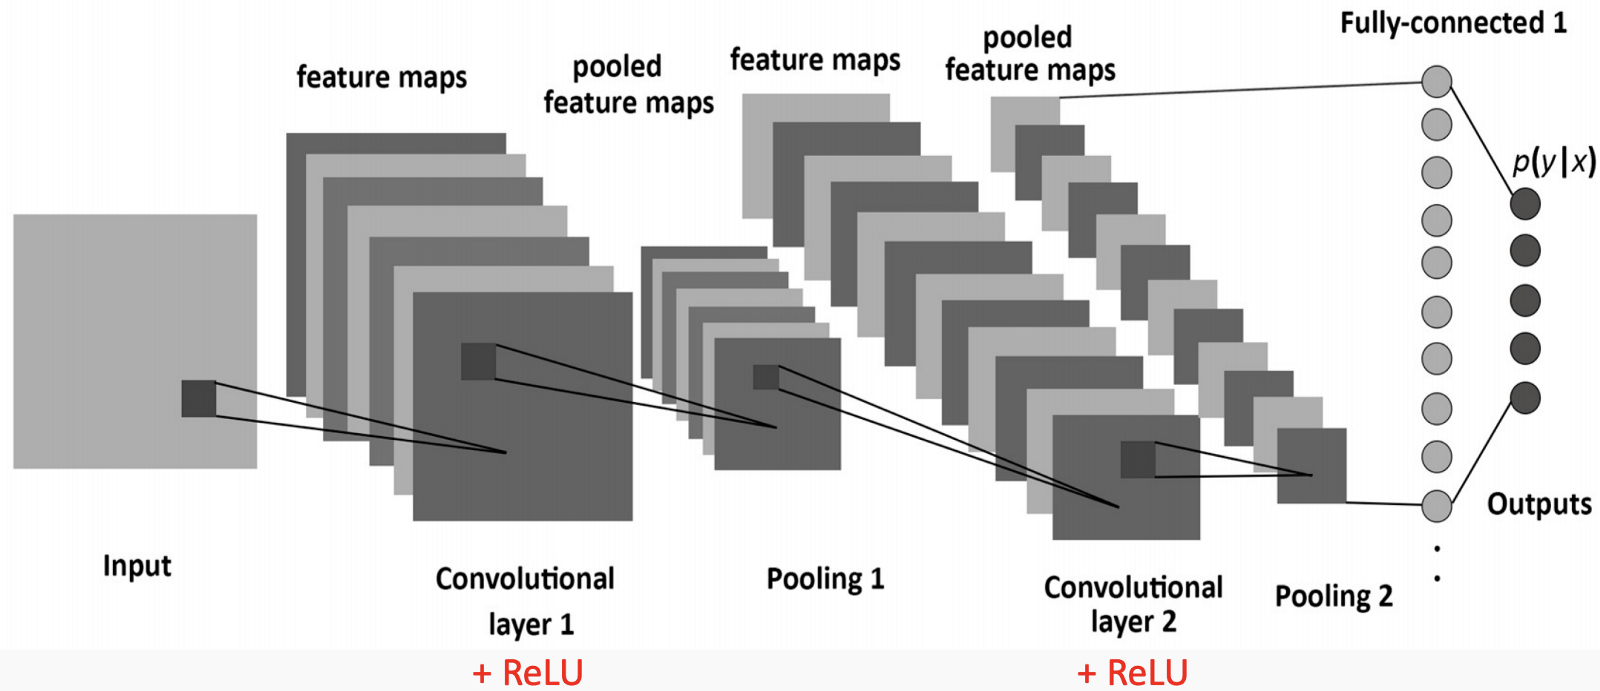
\includegraphics[width=\textwidth/4]{ETH-DS-2020/AML/Resources/cnn.png}
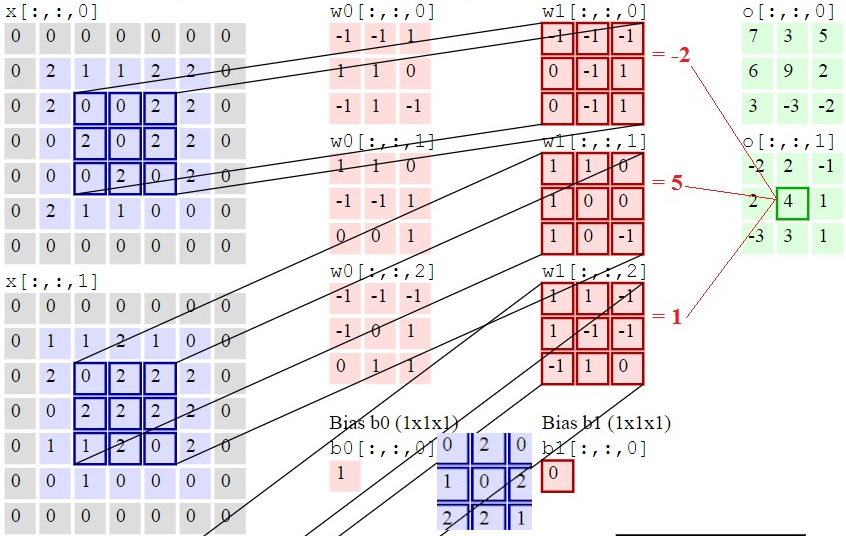
\includegraphics[width=\textwidth/4]{ETH-DS-2020/AML/Resources/conv2.jpg}
\term{Convolutional layer:} Consists of multiple stages\\
\begin{inparaitem}[$\color{mygreen} \triangleright$]
\item Conv stage: $(I*K)[i,j] = \sum_{k=-\infty}^{\infty}\sum_{l=-\infty}^{\infty}I[i-k,j-l] \cdot K[k,l]$ where $K$ is the kernel and $I$ is the 2D input(/image)\\
\item Activation: Apply some activation function\\
\item Pooling: Reduce temporal/spatial dimension (Max/Mean/Sum). To compensate for information loss, apply several kernels in convolution stage.\\
\end{inparaitem}
\term{Properties of convolutional layers:}\\
\textbf{\textcolor{mygreen}{+}} Compute efficient (backprop shares params)\\
\textbf{\textcolor{mygreen}{+}} Translation equivariant (only w.o. pooling!)\\
\textbf{\textcolor{mygreen}{+}} Parameter sharing helps reducing \#params\\
\textbf{\textcolor{red}{-}} Not all data are sequences or translationally equivariant\\
\textbf{\textcolor{red}{-}} Receptive fields are local => hard to connect distant information\\
\term{Output dim:}
$\text{dim}^{\text{out}} = \left \lfloor{\frac{\text{dim}^{\text{in}}+2P-K}{S}}\right \rfloor + 1$; $K$ kernel size, $S$ stride, $P$ padding
%\term{Application areas:}\\
%\begin{inparaitem}[$\color{mygreen} \triangleright$]
%\item Computer vision: Pyramidal structure is very common (increase number of kernels and reduce dimension in every step). Models are very deep and wide\\
%\item Natural language processing: Words first get encoded to feature vectors. Then CNN's can be applied on these vectors. Recently combinations of CNN's and attention and memory units became popular.
%\end{inparaitem}
	\section{Deep Gradients}
\term{Short Connectivity}\\ 
\begin{inparaitem}[$\color{mygreen} \triangleright$]
\item Residual layer (add): Init $f=0$, for $x\in\mathbb{R}^n$ let $g(x):=
\begin{cases}
    x+f(x,\theta) &, n=m\\
    Wx+f(x,\theta)&, n\neq m
\end{cases}
\ \ \in\mathbb{R}^m$\\
Thus, $J_q=I+J_f\approx I$, resp. $J_q=W+J_f\approx W$\\
\item Dense Connectivity/Skip connections (concat.): $\phi(W\lbrack x,f(x,\theta)\rbrack)$
\item DenseNet Block: Layers concatenated with all downstream\\
\term{Batch Normalization}\\
Idea: normalize act. layers and backprop thru\\
Alg: \item Fix layer $l$ \& batch $I\subset [1:s]$
\item $\bs{\mu}^l:=\frac{1}{|I|}\sum_{t\in I}\bs{z}^l[t],$ $\bs{z}^l[t]:=(F^l\circ\cdots\circ F^1)(\bs[t]),$ $\sigma_i^l:=\sqrt{\delta + \frac{1}{|I|}\sum_{t\in I}(z^l_i[t]-\mu_i^l)^2}$,
\item $\bs{\mu}$ and $\bs{\sigma}$ are diffable functions of weights

\item Normalized activities: $\tilde{z}_i^l:=(z_i^l-\mu_i^l)/\sigma_i^l$

\item Regain representational power: $\hat{z}_i^l:=\alpha_i^l\tilde{z}_i^l+\beta_i^l$
(+) esp. effective in vision
(-) depends on batch size, not suitable $\forall$ architectures


\term{Layer Normalization}
\item $\mu^l[t]:=\frac{1}{m^l}\sum^{m^l}_{i=1}z_i^l[t],$ i.e. population average $\sigma_i^l[t]:=\sqrt{\delta + \frac{1}{m^l}\sum^{m^l}_{t=1}(z^l_i[t]-\mu_i^l[t])^2}$
(+) esp. effective in NLP (-) no consistent benefits
\end{inparaitem}
	\section{Regularization}
\term{Def:} Any aspect of learning intended to lower generalization error (but not train. error).

\begin{inparaitem}[$\color{mygreen} \triangleright$]
\term{E.g.} \item Informed reg: prior knowledge \item Simplicity bias: simpler models \item Data augment. \& cross-task learning \item Model averaging, ensemble methods, drop-out
\end{inparaitem}

\subsection*{Norm-based Regularization}
$\mathcal{R}_\Omega(\bs{\theta};\mathcal{S})=\mathcal{R}(\bs{\theta};\mathcal{S})+\Omega(\bs{\theta})$, w. $\mathcal{S}$ train data sample, $\Omega$ functional
\term{E.g.} $\Omega(\bs{\theta})=\frac{1}{2}\sum^L_{l=1}\mu^l||\bs{\Theta}^l||_F^2, \; \mu^l\geq 0$

\term{Weight Decay/$L_2$-regularization:}
$\nabla \Omega=\mu\bs{\theta}$ or $\frac{ \partial\Omega}{\partial \theta^l_{ij}}=\mu\theta^l_{ij}$

Grad. desc. then: $\bs{\theta}(k+1)=(1-\mu\eta)\bs{\theta}(k)-\eta\nabla \mathcal{R}(\bs{\theta}(k))$

Approx: $\mathcal{R}(\bs{\theta})\approx \mathcal{R}(\bs{\theta}^*)+\frac{1}{2}(\bs{\theta}-\bs{\theta}^*)^T\bs{H}_{\theta^*}(\bs{\theta}-\bs{\theta}^*)$

$\nabla \mathcal{R}_{\Omega}=\bs{0}\iff \bs{\theta}=\bs{Q}(\bs{\Lambda}+\mu \bs{I})^{-1}\bs{\Lambda}\bs{Q}^T\bs{\theta}^*,$ w. $\bs{H}=\bs{Q}\bs{\Lambda}\bs{Q}^T$, $\bs{\Lambda}=$diag$(\lambda_1,\dots,\lambda_d)$

\subsection*{Regul via Contrained Optim $\min_{||\bs{\theta}||\leq r}\mathcal{R}(\bs{\theta})$}

\term{Projected Gradient Descent}
$\bs{\theta}(k+1)=\prod_r[\bs{\theta}(k)-\eta\nabla\mathcal{R}(\bs{\theta}(k))],$ w. $\prod_r(\bs{v}):=\min \{a,\frac{r}{||\bs{v}||}\}\bs{v}$

\subsection*{Early Stopping: Equiv to L2 reg w $\lambda=$}
Stop when validation loss flattens.

\subsection*{Ensemble Methods: Bagging}
\term{Bagging:} Combine $k$ models $\bs{\theta}^k$ trained on $r$ bootstrapped samples $\mathcal{S}^k_r\subset \mathcal{S}$ (w replacement)

\term{Prediction:} $p(\bs{y}|\bs{x})=\frac{1}{K}\sum^K_{k=1}p(\bs{y}|\bs{x};\bs{\theta}^k)$

\subsection*{Other Ensembling}
\begin{inparaitem}[$\color{mygreen} \triangleright$]
\item Stochastic model training \item SGD init. \item Different architect.s \& model classes 
\end{inparaitem}

\subsection*{Distillation}
Transfer knowledge from complex (source) model into simpler (target) model.

\term{Blackbox distillation:}
\begin{inparaitem}[$\color{mygreen} \triangleright$]
\item label additional data w source model
\item train target model on augmented data
\item refinement: use soft targets
\end{inparaitem}

\subsection*{Dropout (set weight $i$ to 0 w prob $\pi_i$)}
Realizes ensemble
$p(y|\bs{x})=p\sum_{\bs{Z}}p(\bs{Z})p(y|\bs{x},\bs{Z})$ w. random mask $\bs{Z}$ defining dropbox probabilities $\pi^l_i$

\term{Prediction:} average $\approx10-20$ samples or $\tilde{\theta}_{ij}^l x_j\leftarrow \pi^{l-1}_j\theta_{ij}^l x_j=\E_{\bs{Z}} z^{l-1}_j\theta^l_{ij}x_j$

\term{Thm:} approx. (sometimes exact) to geometrically averaged ensemble


\subsection*{Data Augmentation}
\term{Virtual e.g.s:} $\mathcal{D}^*=\mathcal{D}\cup\{(\tau(\bs{x}),y) : (\bs{x},y)\in\mathcal{D} \}$

$\tau=$ 
\begin{inparaitem}[$\color{mygreen} \triangleright$]
\item Rotation
\item Noise
\item Reflection
\item Color shift
\item Crop
\item PCA component/noise
\item Resize
\end{inparaitem}

\term{Noise Injection}
\begin{inparaitem}[$\color{mygreen} \triangleright$]
\item Inputs \item Weights \item Outputs
\end{inparaitem}

\subsection*{Task Augmentation}
\term{Pre-training}
Initialize weights trained on simple/partial task, fine-tune on full task

\term{SemiSupervised}
\#unlabeled>\#labeled data

Define generative model w log-likelihoods.

Optimize \textbf{additive combination} of supervised and unsupervised risk, while \textbf{sharing parameters}.
(+) More eff. (-) More exp. than pre-training

\subsection*{Multi-Task Learning}
Jointly learn shared low level representations $\forall$ tasks but high level representions per task.
	\section{Recurrent Neural Networks}
\subsection*{Simple RNNs}
\term{Hidden state space sequence:} $\bs{h}^t=F(\bs{h}^{t-1},\bs{x}^t,\bs{\theta}), \; \bs{h}^0=\bs{0},t\leq s$ (Markov P. \& $F\bot t$)

\term{RNN:} $F(\bs{h},\bs{x};\bs{\theta})=\sigma(\bs{W}\bs{h}+\bs{U}\bs{x}+\bs{b})$

Optionally:
$\bs{y}=H(\bs{h};\bs{\theta}):=\sigma(\bs{V}\bs{h}+\bs{c})$

\subsection*{Sequence Loss Function}
\term{Settings:} 1. Normal $L$ for $\bs{h}^T\mapsto H(\bs{h}^T;\theta)=\bs{y}$

2. $\mathcal{R}(\bs{y}^1,\dots,\bs{y}^T)=\sum^T_{t=1} \mathcal{R}(\bs{y}^t)=\sum_{t} \mathcal{R}(H(\bs{h}^t;\theta))$

\begin{multicols}{2}
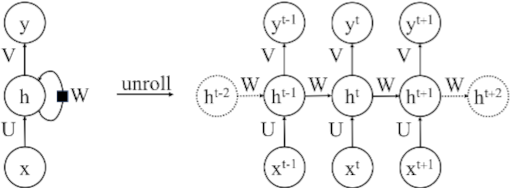
\includegraphics[width=\textwidth/8]{ETH-DS-2020/AML/Resources/unroll_rnn.png}

\term{Variable length noisy memory:} $(\bs{x}^1,\dots,\bs{x}^{t-1})\mapsto\bs{h}^t$
\end{multicols}
\term{Adv. over $T$-node f.c. layer:} param. sharing

\term{Backprop. through time:} $\dot{\sigma}_i^t:=\sigma'(\bar{F}(\bs{h}^{t-1},\bs{x}^t))$

$\frac{\partial\mathcal{R}}{\partial w_{ij}}=\sum^s_{t=1} \frac{\partial\mathcal{R}}{\partial \bs{h}^t_i}\cdot \frac{\partial\bs{h}^t_i}{\partial w_{ij}}=\sum^s_{t=1} \frac{\partial\mathcal{R}}{\partial \bs{h}^t_i}\cdot \dot{\sigma}_i^t \cdot \bs{h}^{t-1}_j$

$\frac{\partial\mathcal{R}}{\partial u_{ik}}=\sum^s_{t=1} \frac{\partial\mathcal{R}}{\partial \bs{h}^t_i}\cdot \frac{\partial\bs{h}^t_i}{\partial u_{ik}}=\sum^s_{t=1} \frac{\partial\mathcal{R}}{\partial \bs{h}^t_i}\cdot \dot{\sigma}_i^t \cdot \bs{x}^{t}_k$

\subsubsection*{$(\bs{y}=\bs{y}^s)$-RNNs/last step RNNs}

$\nabla_{\bs{h}^t} \mathcal{R} =[\prod^s_{r=t+1}\bs{W}^T \bs{S}(\bs{h}^r)]\cdot\bs{J}_H\cdot\nabla_{\bs{y}}\mathcal{R}$

$=[\prod^s_{r=t+1}\bs{W}^T \bs{S}(\bs{h}^r)]\cdot\bs{z},$
w $\bs{S}(\bs{h}^r)=\diag (\dot{\sigma}^r_1,\dots,\dot{\sigma}^r_n)$

$\leq \bs{I}$ for $\sigma\in\{\text{logistic, tanh, ReLu}\}$
\subsubsection*{Vanishing/Exploding Gradients w }
$\sigma_{\max}(\bs{W})<1,\; \bs{S}(\cdot)\leq \bs{I}\implies ||\nabla_{\bs{x}^t}\mathcal{R}||\stackrel{s-t\rightarrow \infty}{\rightarrow}0$

$\sigma_{\max}(\bs{J})>1 \implies$ ``gradients explode''

%$||\prod^s_{r=t+1}\bs{W}^T \bs{S}(\bs{h}^t)||_2
%\stackrel{\text{if }\bs{S}(\cdot)\leq \bs{I}}{\leq}
%||\prod^s_{r=t+1}\bs{W}^T||_2
%\leq
%||\bs{W}||^{s-t}_2
%\leq
%[\sigma_{\max}(\bs{W})^{s-t}]\stackrel{\text{if } \sigma(\bs{W})<1}{\rightarrow}0$ as $s-t\rightarrow \infty$

\begin{multicols}{2}
\term{Reverse order RNNs:}
$\bs{g}^t=G(\bs{x}^t,\bs{g}^{t+1};\bs{\theta})$\\
\term{Bi-directional RNNs:}
see pic (right)

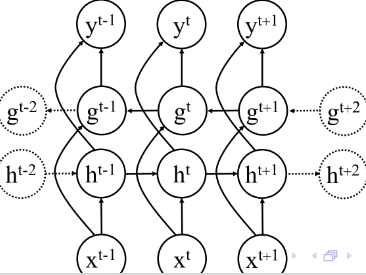
\includegraphics[width=\textwidth/11
]{ETH-DS-2020/AML/Resources/bi-directional.png}
\end{multicols}
\begin{multicols}{2}
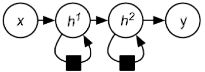
\includegraphics[width=\textwidth/9
]{ETH-DS-2020/AML/Resources/hierarchical2.png}

$\bs{h}^{t,l}=F(\bs{h}^{t-1,l},\bs{x}^{t};\bs{\theta}),\; (l=1,..,L),$ $\bs{y}^t=H(\bs{h}^{t,L};\bs{\theta})$
\end{multicols}
(-) Long term retention vs. short term changes

\subsection*{LSTM}
Forget gate: $\bs{f}_t=\sigma(\bs{W}_f\cdot[\bs{h}_{t-1},\bs{x}_t]+\bs{b}_f)$

Input gate: $\bs{i}_t=\sigma(\bs{W}_i\cdot[\bs{h}_{t-1},\bs{x}_t]+\bs{b}_i)$

Candidate: $\tilde{C}_t=\tanh(\bs{W}_C\cdot [\bs{h}_{t-1},\bs{x}_t]+\bs{b}_C)$

Cell: $\bs{C}_t=\bs{f}_t\odot \bs{C}_{t-1}+\bs{i}_t\odot\tilde{\bs{C}}_t$

Output: $\bs{o}_t= \sigma(\bs{W}_o\cdot[\bs{h}_{t-1},\bs{x}_t]+\bs{b}_o)$

Noisy memory: $\bs{h}_t=\bs{o}_t\odot \tanh(\bs{C}_t)$
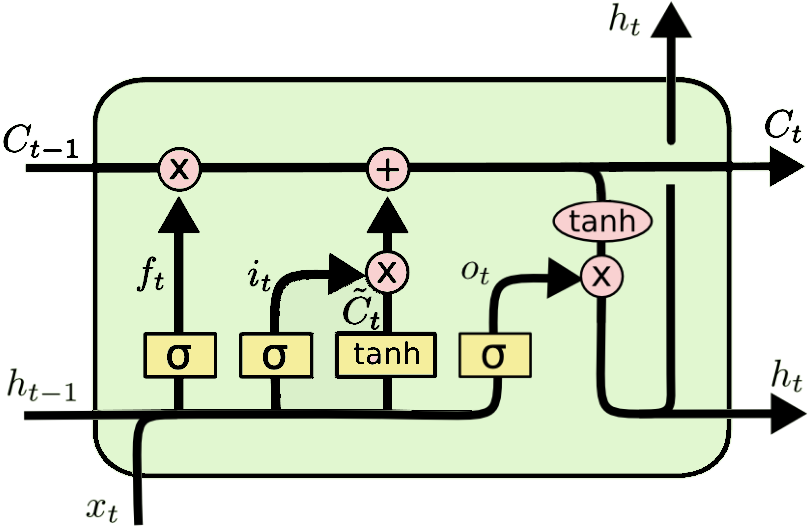
\includegraphics[width=\textwidth/5
]{ETH-DS-2020/AML/Resources/lstm_edited.png}
\subsection*{GRU}
\begin{multicols}{2}
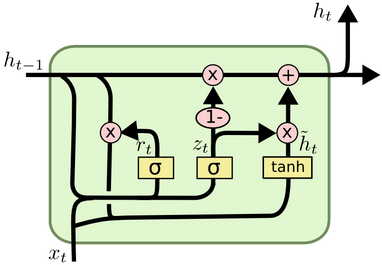
\includegraphics[width=\textwidth/8
]{ETH-DS-2020/AML/Resources/GRU.png}

$\bs{z}_t= \sigma(\bs{W}_z\cdot[\bs{h}_{t-1},\bs{x}_t])$

Remember gate: $\bs{r}_t= \sigma(\bs{W}_r\cdot[\bs{h}_{t-1},\bs{x}_t])$

$\tilde{\bs{h}}_t= \tanh(\bs{W}\cdot[\bs{r}_t\odot\bs{h}_{t-1},\bs{x}_t])$

ConvexOld+New: $\bs{h}_t=(1-\bs{z}_t)\odot\bs{h}_{t-1}
+\tilde{\bs{h}_t}\odot\bs{z}_t$
\end{multicols}

\subsection*{Unsegmented Sequences}
$p(\bs{\pi}|\overrightarrow{x})=\prod^T_{t=1}y_{\pi_t}$ w $\bs{\pi}_t$ label+blank distrib.

$p(\bs{l}|\overrightarrow{x})=\sum_{\pi\in B^{-1}(\bs{l})}p(\bs{\pi}|\overrightarrow{x})$

\subsection*{Learning Sequences}
Learn: $p(\bs{y}^{1:T}|\bs{x}^{1:T})\approx\prod^T_{t=1} p(\bs{y}^t|\bs{x}^{1:t},\bs{y}^{1:t-1})$

Naive RNN: $\bs{x}^{1:t}\stackrel{F}{\mapsto}\bs{h}^t, \bs{h}^t\stackrel{H}{\mapsto}\bs{\mu}^t, \bs{\mu}^t\mapsto p(\bs{y}^t)$

Problem: $p(\bs{y}^t)$ depends on $\bs{y}^{1:t-1}$ only thru $\bs{h}^t$

Cond. $\bot$ assumption: $p(\bs{y}^t|\bs{x}^t,\bs{y}^{1:t-1})=p(\bs{y}^t|\bs{x}^t)$


\begin{multicols}{2}
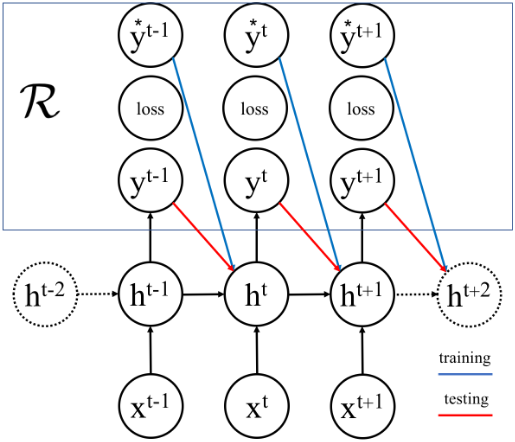
\includegraphics[width=\textwidth/7
]{ETH-DS-2020/AML/Resources/seq_feedback.png}
\term{Output feedback}\\
During train: Teacher forcing\\
(+): improves learn\\
(-): biased training\\
$\; \; \; \;$
\textcolor{red}{Seq2Seq:}\\
$\; \; \; \;$ Encoder-Decoder
\end{multicols}
\textcolor{purple}{Encoder:} $(\bs{x}^1,\dots,\bs{x}^T)\mapsto\bs{z}$ (e.g. RNN w $\bs{z}=\bs{h}^T$)

\color{purple}{Decoder:} $\bs{z}\mapsto(\bs{y}^1,\dots,\bs{y}^S)$ \color{myblue}
(e.g. RNN  output feedback and a stop symbol)

\term{ImageCapt:}Image Enc+Seq2SeqDec+Finetune
	\section{Learning Theory}
\term{Shattering coeff:} $\text{Shatter}(\mathcal{F},s):=\{(f(\bs{x}[1]),\dots,f(\bs{x}[s]))\in \{-1,1\}^s : f\in\mathcal{F})\}$

\term{VC-dim:} $\text{VC-dim}(\mathcal{F}):=\sup \{s:|\text{Shatter}((\mathcal{F},s)|=2^s\}$

\term{VC-ineq:}
$\mathbb{P}\{\sup_{\mathcal{F}} |\hat{l}(f)- \mathbb{E}l(f)|>\epsilon \}\le 8|\text{Shatter}(\mathcal{F},s)|e^{-s\epsilon^2/32}$

Fit $s$ random labels perfectly $\implies \textbf{VC-dim}\ge s$

%\subsection*{PAC-Bayesian thms}
%0-1 loss: $e_f(\bs{x},y)=1\{f(\bs{x}\neq y\}=\frac{1-yf(\bs{x})}{2}$; $e^S_f:=\hat{e}_f$

%Generalization gap:
%$\delta^S_f:=\max(0,e_f-e^S_f)\le |e_f-e^S_f|=:\sqrt{\Delta_f^S}$

%\term{Donsker:} $\forall \mathbb{Q} << \mathbb{P}$, $\mathbb{P}$-measurable $\phi$:

%$\mathbb{E}_{\mathbb{Q}}[\phi]\le KL(\mathbb{Q}||\mathbb{P})+\ln \mathbb{E}_{\mathbb{P}}[e^\phi]$

\term{McAllestor:} $\forall P, Q, \epsilon\in (0,1):$ with prob(S) $\ge\epsilon$:
$\mathbb{E}_{\mathbb{Q}}[e_f]-\mathbb{E}_{\mathbb{Q}}[e_f^S]\le \sqrt{\frac{2}{s}[KL(Q||P)+\ln (\frac{2\sqrt{s}}{\epsilon})]}.$

$\tilde{O}(1/\sqrt{s})$

\term{Spectral complexity}
DNN $\mathcal{A}$, each layer $l$ w weight matrix $W^l$ and Lipschitz const $\rho^l$,
$R(\mathcal{A})=\Big(\prod^L_{l=1}\rho^l||W^l||_2\Big)\Big(\sum^L_{l=1}\frac{||(W^l-M^l)^T||^{2/3}_{2,1}}{||W^l||_2^{2/3}}\Big)^{2/3}.$

\term{Bartlett:} $\forall\mathcal{A},$ margins $\gamma>0:$ w $\text{prob}=1-\delta:$

Test Error($f$)$\le$Empirical $\gamma$-margin Error($f$)

$\tilde{O}\big(\frac{||X||_F R(\mathcal{A}}{\gamma s}\ln(\text{max-width})-\sqrt{\ln\delta/2}\big)$

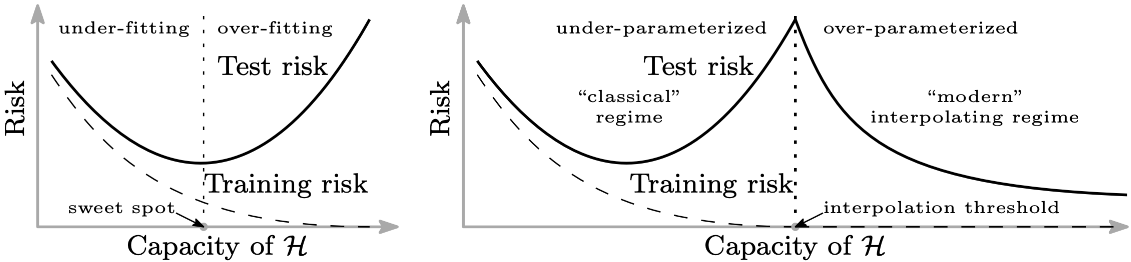
\includegraphics[width=\textwidth/4
]{ETH-DS-2020/AML/Resources/double_descent.png}

\term{Thm:} For any $\epsilon>0,\delta\in (0,1/4]$, when $D=\Omega(\max(m\ln\frac{m}{\delta},m\ln\frac{1}{\epsilon})),\gamma\in[0,1]$, the $\mathcal{L}^{(\gamma)}$ loss, $\epsilon_{\text{unif-alg}}(m,\delta)\ge 1-\epsilon_{\text{gen}}(m,\delta)$.

Uniform convergence:
$\mathbb{P}_{S\sim\mathcal{D}^m}(\sup_{h\in\mathcal{H}}|\mathcal{L}_{\mathcal{D}}(h)-\hat{\mathcal{L}}_S(h)|\le \epsilon_{unif}(m,\delta))\ge 1-\delta$
	\section{$(\mathcal{V},\mathcal{E},\mathcal{W})$-Graph Neural Networks }
\subsection*{Spectral Convolution}
$x:=(v_1,\dots,v_n), n=|\mathcal{V}|,$ incid matr $\nabla\in\mathbb{R}^{|\mathcal{E}|\times |\mathcal{V}|}$

\term{Edge derivative} $``\nabla_{i,j}x''=\frac{\partial}{\partial e_{i,j}}x:=A_{i,j}(x_j-x_i)$

\term{2nd order derivative/Laplacian} $Lx:=\nabla^T\nabla x$

\term{Diagonal degree matr.} $D_{ii}:=\sum_j A_{i,j}$, $D_{i\neq j}=0$

\term{Corollary} $L=D-A$

\term{Normalized Laplacian} $L'=I-D^{-1/2}AD^{-1/2}=D^{1/2}LD^{1/2}$ (in practice use this since $\lambda_i\le 2$).

$L=\nabla^T\nabla$ sym. pos. def. $\implies L=U\Lambda U^T$.

\term{Graph Fourier basis trafo:} $\hat{x}=U^Tx$, $x=U\hat{x}$

\term{Spectral Graph Convol.:} $h(L)x:=Uh(\Lambda)U^Tx$
\term{Comp Complexity of ":} $\mathcal{O}(|\mathcal{V}|^3)$

\term{Trick, use polys:} $p(t)=\sum^K_{i=0}\alpha_i t^i$

\term{Filtering operation:}
$p(L)x:=Up(\Lambda)U^Tx=U\Big(\sum^K_{i=0}\alpha_i\Lambda^i\Big)U^Tx=\sum^K_{i=0}\alpha_i L^i$

\term{Comp Complexity of " (if $L$ sparse):} $\mathcal{O}(|\mathcal{E}|)$

\term{In practice:}
\begin{inparaitem}[$\color{mygreen} \triangleright$]
\item Learn $c_{in}\cdot c_{out}$ polynomial kernels $p_{i,j}(t)=\sum^K_{k=0}\alpha_{i,j,k}t^k$
\item add bias $\beta_j$
\item sum over $c_{in}$ input channels
\end{inparaitem}

\term{Graph Convolution Layer:} Input $X^i_{in}\in\mathbb{R}^n$ (channel $i$), output:
$X^j_{out}=\sum^{c_{in}}_{i=1}p_{i,j}(L)X^i_{in}+b_j$.

\term{\#params:} $c_{in} \cdot c_{out}\cdot (K+1)+c_{out}$

\term{ChebNet:} \begin{inparaitem}[$\color{mygreen} \triangleright$]
\item Learn Chebyshev polys for scalability+stablity
\item Graph coarsening
\end{inparaitem}

\subsection*{Vertex Convolution/GNN}

\begin{inparaitem}[$\color{mygreen} \triangleright$]
\item \term{Shared edge operation:} $e(X^{(k)}_i,X^{(k)}_j,A_{i,j})$
\item \term{Shared node operation:} $h(X^{(k)}_i)$
\item aggregation $\text{AGG}$ + combination $\text{COMB}$ funcs
\end{inparaitem}

$Z^{(k)}_i=\text{AGG}(\{e(X^{(k)}_i,X^{(k)}_j,A_{i,j}):v_i\sim v_j\})$

$X^{(k+1)}_i=\text{COMB}(Z^{(k)}_i,h(X^{(k)}_i))$

\subsection*{1st order spectral convolution/GCN}
\term{Simultaneous activity propagation:}

$\bs{X}^{l+1}=\sigma( \bs{W}^{l}\bs{X}^{l}\bs{Q} )$ ($\bs{W}\bs{X}$ along dimensions, $\bs{X}\bs{Q}$ along datapts), $\tilde{\bs{A}}:=\bs{A}+\bs{I}$,
$\bs{Q}=\tilde{\bs{D}}^{-1/2}\tilde{\bs{A}}\tilde{\bs{D}}^{-1/2}$, diagonal degree $\tilde{\bs{D}}$ of $\tilde{\bs{A}}$, i.e. 
$q_{ij}=\frac{a_{ij}+\delta_{ij}}{\sqrt{\tilde{d}_{i}\tilde{d}_{j}}}, \tilde{d}_{i}=1+\sum_j A_{ij}, \delta_{ij}=1\{i=j\}$

$(\bs{X}^l\bs{Q})_{ij}=([\bs{x}^l[1],\dots,\bs{x}^l[n]]\cdot \bs{Q})_{ij}=\sum^n_{k=1}x_{ik}q_{kj}$

%\textcolor{red}{Emmanuel TODO: probably should add ``justifying GCNs'' slides}
	\section{Adversarial Examples}

\subsection*{Why care about adv examples?}
\begin{inparaitem}[$\color{mygreen} \triangleright$]
\item \term{Security/Safety:} ex:self-driving cars
\item \term{o.o.d generalization:} ex: faulty camera creates noise in image
\item \term{understanding bias} ex: ai changes decision solely based on gender
\end{inparaitem}

\subsection*{Minimal adversarial perturbation} Let $NN: \mathbb{R}^d \rightarrow \{1,..,C\} $ be a c-classifier and $x \in \mathbb{R}^d$ be an input. Then find $r \in \mathbb{R}^d$ such that \begin{inparaitem}[$\color{mygreen} \triangleright$]
\item $NN(x+r) \ne NN(x)$
\item $||r||_p$ is small/minimized
\end{inparaitem}
%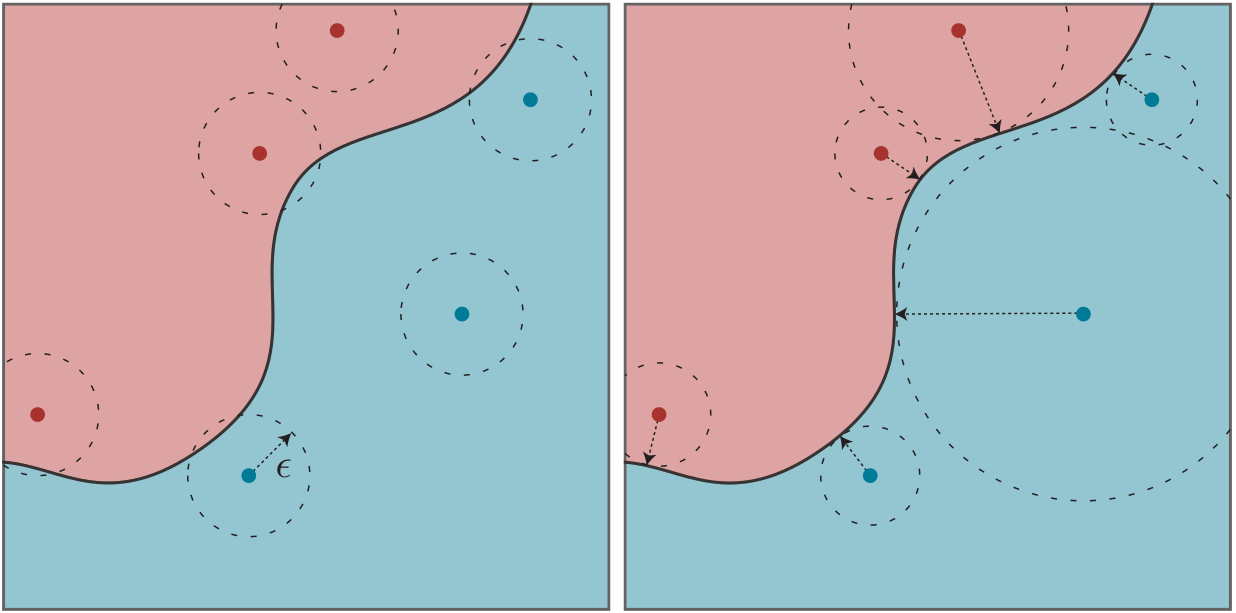
\includegraphics[width=\textwidth/4]{ETH-DS-2020/AML/Resources/adv_examples.png}
\subsection*{Measuring adversarial robustness} 2 equiv. robust defs:
\begin{inparaitem}[$\color{mygreen} \triangleright$]
\item Fraction of $x\in\mathcal{D}$ s.t. $\forall r, ||r||_p \le \epsilon: NN(x) = NN(x+r)$
\item Average norm $||r||_p$ for which $NN(x+r) \ne NN(x)$
\end{inparaitem}

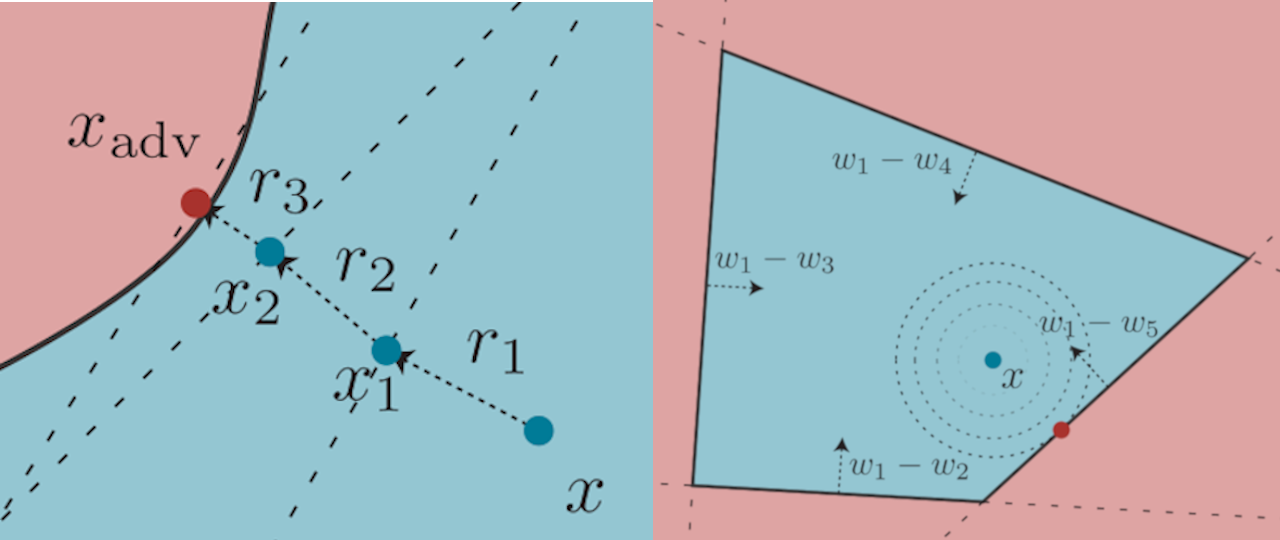
\includegraphics[width=\textwidth/5]{ETH-DS-2020/AML/Resources/adv_examples3.png}
\subsection*{Find adv. perturbation of linear classifier}Given a simple linear classifier $f: \mathbb{R}^d \rightarrow [C],\  f(x) = W^Tx + b$, where $W = [w_1,...,w_c],\ w_i \in \mathbb{R}^d$, $x \in \mathbb{R}^d$ and $f(x) = 1$ the minimal perturbation $r^*$ is:
$r^* = \arg\min_{r_i,\ i\ne 1} ||r_i||_2$ where $r_i = \frac{f_1(x) - f_i(x)}{||w_i - w_1||_2^2}(w_i - w_1)$ (see right image)

\subsection*{Find adv. perturbation of general classifier}Given a general classifier $f: \mathbb{R}^d \rightarrow [C],\ x_0 \in \mathbb{R}^d$ and $f(x_0) = 1$ Idea: Linearize classifier, then iteratively apply solution of linearized classifier problem (see left image). Compute $r^{(i+1)} := \arg\min_{r_k^{(i+1)}} ||r_k^{(i+1)}||$ s.t.\linebreak $(\nabla_x f_1(x_i) - \nabla_x f_k(x_i))^T r_k^{(i+1)} + f_1(x_i) - f_k(x_i)\ <\ 0$\linebreak
and then update $x_{i+1} = x_i + r^{(i+1)}$

\subsection*{Adversarial training} Define robust training procedure:\\ $\min_\theta\max_{||r||_p \le \epsilon}loss(f_\theta(x+r), y)$.\\ Alternately max and min:
\begin{inparaitem}[$\color{mygreen} \triangleright$]
\item Initialize $\theta_0$

\item \term{Maximization step:}

$r^{t+1}(\theta^t) = \arg\max_{||r||_p \le \epsilon} loss(f_{\theta^t}(x+r),y)$\\
\item \term{Minimization step:}

$\theta^{t+1}(r^{t+1}) = \theta^{t} - \eta \nabla_\theta loss(f_{\theta^t}(x+r^{t+1}),y)$
\end{inparaitem}

\subsection*{Projected gradient descent} Solves maxation step in adv training. \term{PGD($n$)} computes $r$ in $n$ steps. For $p = 2$, compute:\\
$\Tilde{r}^{s+1} = r^s + \alpha \nabla_x loss(f_\theta(x + r^s), y)$\\
For $p = \infty$, compute: \\
$\Tilde{r}^{s+1} = r^s + \alpha \cdot sign(\nabla_x loss(f_\theta(x + r^s), y))$\\
Finally, project the resulting perturbation back to the $\epsilon - l_p$ ball:
$r^{s+1} = \Pi_\epsilon^p(\Tilde{r}^{s+1})$\\
A special case is the \term{Fast gradient sign method (FGSM)} which computes only 1 step of PGD (with $p = \infty$) without the projection step. However, this attack is weaker

\subsection*{Undesired side-effects of adversarial training:}
\begin{inparaitem}[$\color{mygreen} \triangleright$]
\item \term{Gradient masking:} the gradient (w.r.t. input) norm becomes too small for training samples ($||\nabla_xf(x)||_p \approx 0$)\\
\item \term{Gradient obfuscation:} The gradient (w.r.t.) input becomes extremely noisy (i.e. spiky) or even undefined
\end{inparaitem}
	\section{Memory and Attention}
\term{Memory Networks}
Recursive associative recall: find best memory cell $i$ for query $q$, use content $m_i$ and $x$ to generate next query 
\subsection*{Self-Gated Attention}
\term{Softmax Gating Function:}
$f_{\phi}(\bs{\xi},\bs{h}^1_e,\dots,\bs{h}^s_e)=\frac{1}{\sum_j \exp [\phi(\bs{\xi},\bs{h}^j_e)] }(\bs{h}^1_e,\dots,\bs{h}^s_e)^T,$ query vector $\bs{\xi}\in\mathbb{R}^n$, similarity $\phi:\mathbb{R}^n\times\mathbb{R}^m\rightarrow\mathbb{R}$ (e.g. $n=m$: $\bs{\xi}\cdot \bs{h}_e$)

\term{Transfer-Func:} $F(\bs{\xi},\bs{h}^{1:s}_e)=[\bs{h}^1_e\cdot\cdot\bs{h}^s_e]\cdot f_{\phi}(\bs{\xi},\bs{h}^{1:s}_e)$

Hidden encoding/attending RNN: $(h_e^1,\dots,h^s_e)$

Query from decoding RNN: $(\xi^1,\dots,\xi^s)$

Self-gated attention read-outs: $(\bs{z}^1,\dots,\bs{z}^t)$

Decoding RNN: $(\bs{h}^r_d,\bs{z}^r)\mapsto \bs{h}^{r+1}_d$

\subsection*{Transformers $(d:=d_{\text{model}},h:=\#\text{heads})$}

\term{Self-Attent:}
$W^Q,W^K\in \mathbb{R}^{d\times d_k},W^V\in \mathbb{R}^{d \times d_v}$

$\{Q,K\}=XW^{\{K,Q\}}\in \mathbb{R}^{T\times d_k},V=XW^V\in \mathbb{R}^{T\times d_v}$ 

$\textbf{Att}(Q,K,V)=\text{softmax}(QK^T/\sqrt{d_k})V$

$\term{MultiHead}(Q,K,V):=[\text{head}_1,\dots,\text{head}_h]W^O$,
$\text{head}:=\text{Att}(QW^Q_i,KW^K_i,VW^V_i),W^O\in \mathbb{R}^{hd_v\times d}$

\term{Ex/Alt:} $W^{\{Q,K,V\}}\in\mathbb{R}^{d\times h d_{\{k,v\}}}$, MH=sm$(QK^T)V$

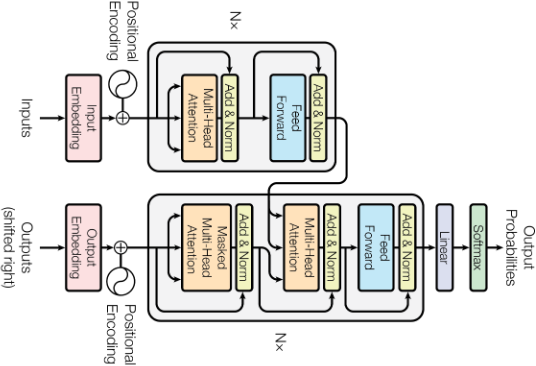
\includegraphics[width=\textwidth/5]{ETH-DS-2020/AML/Resources/transformer2.png}

$\text{FFN}(x_i)=\max(0,x_i W_1+b_1)W_2+b_2$










\iffalse

\term{Key-Value Atten.:}
Item $i$, key $\bs{x}^i$ + value $\bs{z}^i$ embedding:
$F(\bs{\xi},\bs{x}^{1:s},\bs{z}^{1:s})=[\bs{z}^1,\dots,\bs{z}^s]\cdot f(\bs{\xi},\bs{x}^{1:s})$

\term{Scaled Dot-Product Attention} As above w
$f(\bs{\xi})=\frac{\bs{\xi}\cdot\bs{x}}{\sqrt{n}},\; \bs{\xi},\bs{x}\in\mathbb{R}^n$ (or: $\softmax(\frac{QK^T}{\sqrt{d_k}})V$)

\term{Multi-Headed Attention}
$G(\bs{\xi},(\bs{x}^t,\bs{z}^t)^s_{t=1})=\bs{W}[F_1(\bs{\xi},\bs{x}^t,\bs{z}^t),\dots F_h(\bs{\xi},\bs{x}^t,\bs{z}^t)]^T,$
w $F_j(\bs{\xi},\bs{x}^t,\bs{z}^t)=F(\bs{W}^q_j\bs{\xi},\bs{W}^x_j\bs{x}^t,\bs{W}^z_j\bs{z}^t)$ for $j\leq r$ are key-value attention maps (dot-prod)

($\text{Concat}(\text{head}_1,\dots,\text{head}_h)W^O$ w $\text{head}_i=\text{Attention}(QW^Q_i,KW^K_i,VW^V_i)$ and $W^Q_i,W^K_i\in\mathbb{R}^{d_{\text{model}}\times d_k},W^V_i\in\mathbb{R}^{d_{\text{model}}\times d_v}$)

%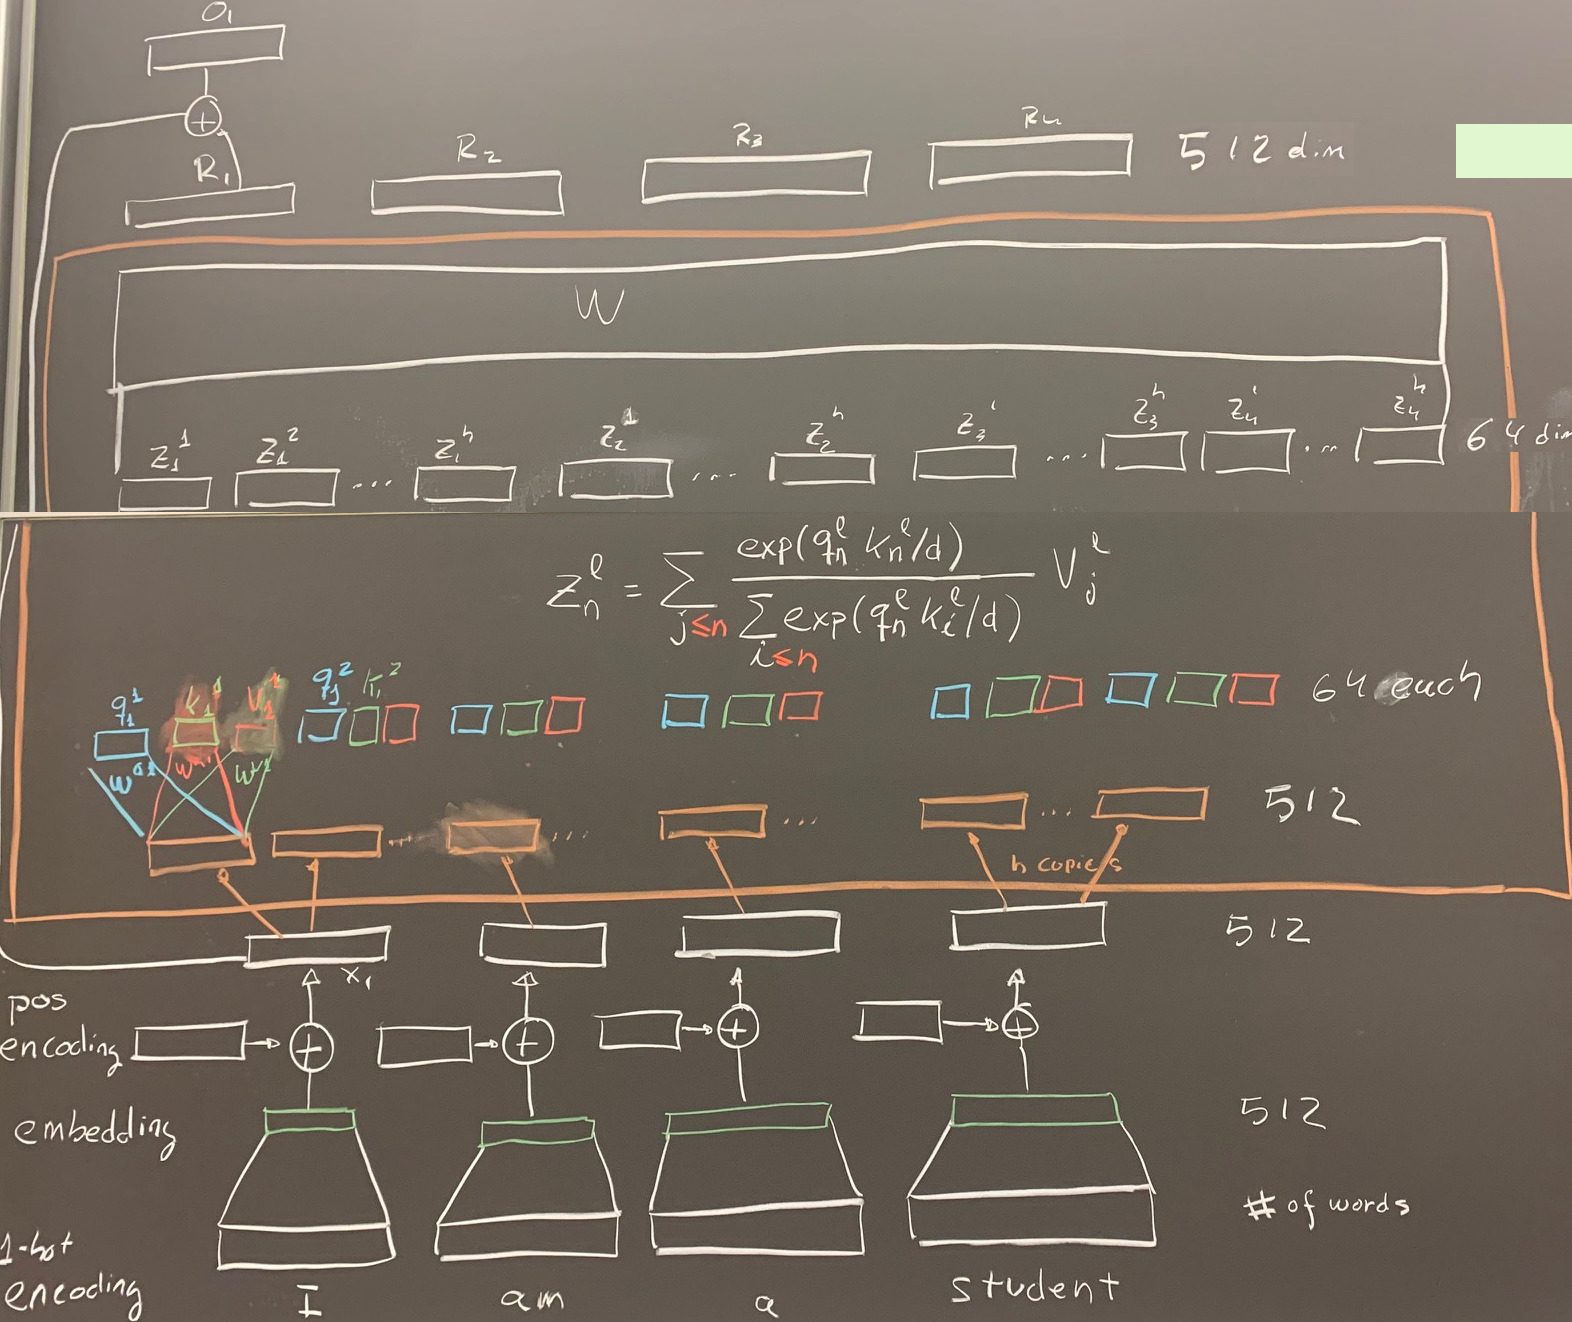
\includegraphics[width=\textwidth/4]{ETH-DS-2020/AML/Resources/transformer.jpg}
 
\fi
	\section{Variational Autoencoder}
\subsection*{Linear Autoencoder}
\term{Goal}: $\text{min}_{\mathbf{E}, \mathbf{D}} ||\mathbf{X} - \mathbf{D}\mathbf{E} \mathbf{X}||^2_F$, w $\mathbf{X} (d \times n),\mathbf{D} (h \times d),\mathbf{E} (d \times h), h < d$.
$\mathbf{E}^{\star} = (\mathbf{A}^{-1})\mathbf{U}_k^{\top}$, $\mathbf{D}^{\star} = \mathbf{U}_k (\mathbf{A}), \forall\mathbf{A}\in\text{GL}(h)$ and $\mathbf{X} = \mathbf{U}\mathbf{\Sigma}\mathbf{V}^{\top}$.
Only convex in $\mathbf{D}$, $\mathbf{E}$ individ.
\term{Eck-Yung:} $X_k=\argmin_{\text{rank}Y\leq k}||X-Y||_F=U\Sigma_k V^T$.

\subsection*{Factor Analysis}
Idea: Assume that (highly) correlated random vec. $x \in \mathbb{R}^n$ can be described by smaller latent vec. $z \in \mathbb{R}^m$ with $m < n$.
%\subsubsection*{Latent variable Models}
%Marginal likelihood: $p(x)=\int p(z)p(x|z)\mu(dz)$

\subsubsection*{Linear Factor Analysis}
Prior: $z\sim \mathcal{N}(0,I)$; Linear observ. model (\term{Decoder: $z \rightarrow x$}): $x=\mu+Wz+\eta,$ w $ \eta\sim\mathcal{N}(0,\Sigma),\Sigma:=\text{diag}(\sigma^2_1,\dots,\sigma^2_n), \eta\perp z; x\in\mathbb{R}^n,\hat{\mu}=\frac{1}{N}\sum^N_{i=1}x_i$

$\implies x\sim\mathcal{N}(\mu,WW^T+\Sigma)$
\term{Pf:} Mom. gen. funcs
\term{Corollary:} only identifiable up to orth. transf.

\subsubsection*{Posterior Inference (Encoder: $x \rightarrow z$)}
Posterior: $\mathcal{N}(\mu_{z|x},\Sigma_{z|x})$; $\mu_{z|x}=W^T(WW^T+\Sigma)^{-1}(x-\mu)$; $\Sigma_{z|x}=I-W^T(WW^T+\Sigma)^{-1}W$
Assume that $\Sigma = \sigma^2 I$. Then for $\sigma^2 \rightarrow 0$ $W^T(WW^T+\Sigma)^{-1} \rightarrow W^\dagger$ and therefore $\mu_{z|x} \rightarrow W^\dagger(x-\mu),\ \Sigma_{z|x} \rightarrow \textbf{0}$. Easy to compute! Otherwise use MLE.
\subsection*{Variational Autoencoders}Same as factor analysis but enc., dec. are DNNs. But, using MLE by maximizing $\log(p(x;\theta)$ doesn't work bec. $p(x;\theta)$ is hard to compute! $\Rightarrow$ Maximize lower bound of $\log(p(x;\theta))$!
\subsubsection*{Decoder $\hat{x}=F^{L:1}(z)$ taking  $z\stackrel{iid}{\sim}\mathcal{N}(\mu,\Sigma)$} 
\term{ELBO}(Evidence lower bound):

$\log p(x;\theta)=\log\int q(z)[p(x|z;\theta)\frac{p(z)}{q(z)}]dz
\stackrel{\text{Jensen}}{\ge} \int q(z)\log p(x|z;\theta)dz-KL(q||p)=\mathcal{L}(\theta,q;x)$
for \term{\textit{any}} distr. $q(z|x)$. Represent $q(z|x)$ as DNN $enc_\phi: x \mapsto (\mu(x), \Sigma(x))$. Then, $z \sim \mathcal{N}(\mu(x), \Sigma(x))$.

\term{Optimizing Var. Autoenc.} Goal, maximize:
$\mathcal{L}(\theta, \phi;X)$. with $enc_\phi: x \mapsto (\mu(x), \Sigma(x))$, $dec_\theta: z \mapsto x$ where $z \sim \mathcal{N}(\mu(x), \Sigma(x))$.\\
\term{Optimizing $dec_\theta$: } Sample $z \sim \mathcal{N}(\mu(x), \Sigma(x))$. Perform backprop. with SGD, treating $z$ as const.\\
\term{Optimizing $enc_\phi$: }Repara. trick: $z \sim \mathcal{N}(\mu(x), \Sigma(x))$ is equiv to $z = \mu(x) + \Sigma(x)^{\frac{1}{2}}\eta$ with $\eta \sim \mathcal{N}(0, I)$. Then, do backprop through $\mu(x), \Sigma(x)$
%Aim: $\hat{\theta}=\argmax_{\theta} \sum_i \mathcal{L}(\theta,q(\cdot;\bs{x}_i);\bs{x}_i))$
%\term{Variational Family} $q(z;x)=p(z|x)$ intractible $\implies$ restrict $q$ e.g. $z\sim\mathcal{N}(\mu(x),\text{diag}(\sigma_1^2(x),\dots,\sigma_n^2(x)))$
%\term{Optimization:} Repara $z=\mu+\Sigma^{1/2}\eta,\eta\sim\mathcal{N}(0,I)$ backprop over $\mu,\Sigma$ for fixed $\eta=\eta(x)$
%\textcolor{red}{TODO:resolve confusion slide 32 from 17a vs. slides 38-39 from 18a}
\term{Thm:} $\nabla_{\mu}\mathbb{E}[f(z)]=\mathbb{E}[\nabla_z f(z)],\; \nabla_{\Sigma}\mathbb{E}[f(z)]=0.5\cdot\mathbb{E}[\nabla_z^2 f(z)]$
%\term{Naïve MC:} $\nabla_{q_{\phi}(z)}\mathbb{E}[f(z)]=\mathbb{E}[f(z)\nabla_{q_{\phi}(z)}q_{\phi}(z)]\approx \frac{1}{L}\sum^L_l$



	\section{Generative Adversarial Networks}
\subsection*{Density Estimation}
Gen.M:$p(x)$, para.M: $p_{\theta}(x)$, Goal: $p_{\theta}(x)=p(x)$.

But:Colps:$p(x)>>p_{\theta}(x)\stackrel{>}{\approx}0$, bad $\mathcal{D}$: $p(x)>>p_{\theta}(x)\stackrel{>}{\approx}0$, norm./integr. (-> EM). MLE:$\hat{\theta}=\text{amax}_{\theta} \mathbb{E}_{x\sim p}[\ln p_{\theta}(x)]\approx \text{amax}_{\theta} \frac{1}{L}\sum\ln p_{\theta}(x)$

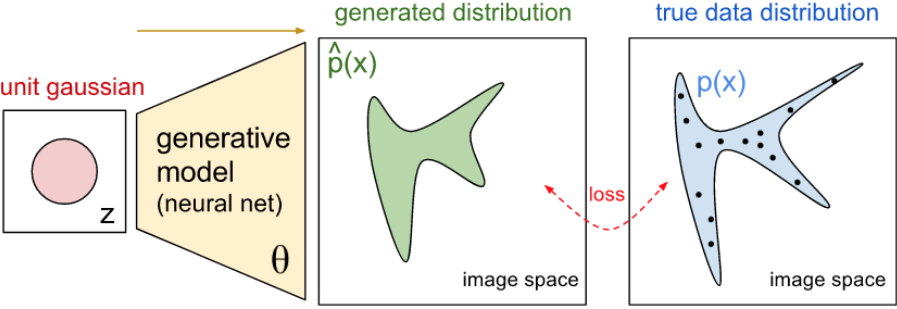
\includegraphics[width=\textwidth/6]{ETH-DS-2020/AML/Resources/gans.png}

$z\sim f$ (rand), $x=NN_{\theta}(z)$ (det)

Likelihood based GANs: opt $\log p(x)$ 

\subsection*{GANs (1. Generate, 2. Classify: Real 1/Fake 0)}
G.f.'14: 
1.$\tilde{p}_{\theta}(x,y)=\frac{1}{2}(y p(x)+(1-y)p_{\theta}(x))$

2.BayesOptClas: $q_{\theta}(x)=\frac{p(x)}{p(x)+p_{\theta}(x)}=P(y=1|x)$

3.$l^*(\theta)= \E_{\tilde{p}_{\theta}}[y\ln q_{\theta}(x)+(1-y)\ln(1-q_{\theta})]$

4. BOC=?, so $q_{\theta}\rightarrow q_{\phi}$ \& $l^*(\theta)\rightarrow \sup_{\phi} l(\theta,\phi)$:

$l^*(\theta)\ge\sup_{\phi}\E_{\tilde{p}_{\theta}}[y\ln q_{\phi}(x)+(1-y)\ln(1-q_{\phi}(x))]$

5.Sadl:$\argmin\{\sup_{\phi} l(\theta,\phi)\}$, so SGD may $\rightarrow \infty$

$(\theta,\phi)^{t+1}=(\theta,\phi)^t+\eta(- \nabla_{\theta} l(\theta^t,\phi^t), \nabla_{\theta}l(\theta^{t+1},\phi^t))$

$\min\limits_G\max\limits_D \E_{x\sim\mathcal{D}}\log D(x)+\E_{z\sim p_z}\log(1-D(G(z)))$

Chllng:Qual ctrl;Trd-of: noisy vs. mode drop

Gf. GAN '14 <DC GAN: Radford '15 < Prog.-Grow. GAN: NVIDIA '18 < CycleGAN

COV (w $f_{\theta}=g_{\theta}^{-1}$): $p_X(x)=p_Z(f(x))|\det (\frac{\partial f_{\theta}(x)}{\partial x^T})|$

Opt: $\min_{\theta}\E[-\log(p_{\theta}(x))]$;
\term{Normalizing flows:} bij. $F$ s.t. eval, invert and $|\det(\partial F)|$ easy 

$F^{-1}=F_1^{-1}\circ\cdots\circ F_L^{-1}$, $\det (\partial F)=\prod^1_{l=L}\det(\partial F_l\circ F_{l-1:1})$, $\det(\partial F^{-1})=\det(\partial F)^{-1}$

Log-likelihood: $ p_X(x) = \text{log}(p_Z(F(\mathbf{x})))  - \sum^L_{l=1}\log|\det(\partial F_l\circ F_{1:l-1})|$

SimpTrafo: $y_{d+1  :D}=x_{d+1:D}\odot\exp s(x_{1:d})+t(x_{1:d})$

%\textcolor{red}{Not sure what to add about "factoring out" and "Glow" etc, slides 31+}
	%$h_{f,t}=\bar{F}_b(x_t,h_{b,t+1};\theta)$, $h_{f,t}=\bar{F}_f(x_t,h_{f,t-1};\theta)$, $y_{t}=G(h_{f,t},h_{b,t})$,
%$\frac{\partial L}{\partial \theta}\imples \sum$
3D-Conv:$O(n,m,k,l)=\sum _c \sum_u\sum_v\sum_w I(x-u,y-v,z-w,c)F_l(u,v,w)$
	
% -*- root: Main.tex -*-

%\subsection{Misc}
%\textbf{Lagrangian:} $f(x,y) s.t. g(x,y) = c$\\
%$
%\mathcal{L}(x, y, \gamma) = f(x,y) - \gamma ( g(x,y)-c)
%$\\
%\textbf{Parametric learning}: model is parametrized with a finite set of parameters, like linear regression, linear SVM, etc. \\
%\textbf{Nonparametric learning}: models grow in complexity with quantity of data: kernel SVM, k-NN, etc.\\
%\textbf{Empirical variance}: Look for dense and sparse regions. Regularize so that sparse regions are not contained (decr. variance). Measure by Variance CV of some classifiers.

% -*- root: Main.tex -*-
%\section{Ensemble Methods}
%Use combination of simple hypotheses (weak learners) to create one strong learner.
%
%strong learners: minimum error is below some $\delta < 0.5$
%
%weak learner: maximum error is below $0.5$
%\begin{equation}
%f(x) = \sum_{i=1}^{n} \beta_i h_i(x)
%\end{equation}
%\textbf{Boosting}: train on all data, but reweigh misclassified samples higher.
%
%\subsubsection*{Decision Trees}
%\textbf{Stumps}: partition linearly along 1 axis\\
%$h(x) = sign(a x_i - t)$\\
%\textbf{Decision Tree}: recursive tree of stumps, leaves have labels. To train, either label if leaf's data is pure enough, or split data based on score.
%
%
%\subsubsection*{Ada Boost}
%Effectively minimize exponential loss.\\
%$f^*(x) = \argmin_{f\in F} \sum_{i=1}^{n} \exp(-y_i f(x_i))$\\
%Train $m$ weak learners, greedily selecting each one
%\begin{equation*}
%(\beta_i, h_i) = \argmin_{\beta,h} \sum_{i=1}^{n} \exp(-y_i (f_{i-1} (x_j) + \beta h(x_j)))
%\end{equation*}
%\begin{compactdesc}
%	\item $c_b(x) \text { trained with } w_i$ \\
%	\item $\epsilon_b = \sum\limits_i^n \frac{w_i^b}{\sum\limits_i^n w_i^b} I_{c(x_i) \neq y_i} $\\
%	\item $\alpha_b = log \frac{1-\epsilon_b}{\epsilon_b} $\\
%	\item $w^{b+1}_i = w^b_i \cdot exp(\alpha_b I_{y_i \neq c_b(x_i)})$
%\end{compactdesc}
%
%Exponential loss function
%
%Additive logistic regression
%
%Bayesian approached (assumes posteriors)
%
%Newtonlike updates (Gradient Descent)
%
%If previous classifier bad, next has heigh weight



%\subsubsection*{Fischer's Linear Discriminant Analysis (LDA)}
%Idea: project high dimensional data on one axis.
%
%Complexity: $\mathcal{O}(d^2n$ with $d$ number of classifiers\\
%$c=2, p=0.5, \hat{\Sigma}_- = \hat{\Sigma}_+ = \hat{\Sigma} \\
%y = sign(w^\top x + w_0) \\
%w = \hat{\Sigma}^{-1}(\hat{\mu}_+ - \hat{\mu}_-) \\
%w_0 = \frac{1}{2}(\hat{\mu}_-^\top \Sigma^{-1} \hat{\mu}_- - \hat{\mu}_+^\top \Sigma^{-1} \hat{\mu}_+)
%$

% -*- root: Main.tex -*-
%\section{Unsupervised Learning}
%\subsection*{Parzen}
%$
%\hat{p}_n = \frac{1}{n} \sum\limits_{i=1}^n \frac{1}{V_n} \phi(\frac{x-x_i}{h_n})
%$
%where $\int \phi(x)dx = 1$
%\subsection*{K-NN}
%$
%\hat{p}_n = \frac{1}{V_k} \text{ volume with } k \text{ neighbours}
%$
%\subsection*{K-means}
%$
%L(\mu) = \sum_{i=1}^{n} \min_{j\in\{1...k\}} \|x_i - \mu_y \|_2^2
%$\\
%
%\textbf{Lloyd's Heuristic}:\\ (1) assign each $x_i$ to closest cluster \\
%(2) recalculate means of clusters.
%
%Iteration over (repeated till stable):
%\begin{compactdesc}
%	\item[Step 1:]$ \text{argmin}_c ||x-\mu_c||^2$ \\
%	\item[Step 2:]$ \mu_\alpha = \frac{1}{n_\alpha} \sum \vec{x}$
%\end{compactdesc}

% -*- root: Main.tex -*-

%\section{Hidden-Markov model}
%State only depends on previous state.
%
%Always given: sequence of symbols $\vec{s} = \{s_1,s_2, \ldots s_n\}$
%\subsection*{Evaluation (Forward \& Backward)}
%Known: $a_{ij}, e_k(s_t)$
%
%Wanted: $P(X = x_i | S = s_t)$
%\begin{eqnarray}
%f_l (s_{t+1}) = e_l(s_{t+1}) \sum f_k(s_t) a_{kl} \\
%b_l(s_t) = e_l(s_t) \sum b_k(s_{t+1}) a_{lk} \\
%P(\vec{s}) = \sum_k f_k(s_n) a_k \cdot \text{ end} \\
%P(x_{l,t} | \vec{s}) = \frac{f_l(s_t) b_l(s_t)}{P(\vec{s})}
%\end{eqnarray}
%Complexity in time: $\mathcal{O}(|S|^2 \cdot T)$

%\subsection{Learning (Baum-Welch)}
%Known: only sequence and sequence space $\Theta$
%
%Wanted: $a_{ij}, e_k(s_t)$ \& most likely path $\vec{x} = \{x_1,x_2,\ldots x_n\}$
%
%\textbf{E-step I:} $f_k(s_t), b_k(s_t)$ by forward \& backward algorithm
%
%\textbf{E-step II:}
%\begin{eqnarray}
%P(X_t = x_k, X_{t+1} = x_l | \vec{s}, \Theta) = \\
%\frac{1}{P(\vec{s})} f_k(s_t) a_{kl} e_l(s_{t+1}) b_l(s_{t+1}) \\
%A_{kl} = \sum\limits_{j=1}^m \sum\limits_{t=1}^n P(X_t = x_k, X_{t+1} = x_l | \vec{s}, \Theta)
%\end{eqnarray}
%\textbf{M-step :}
%\begin{eqnarray}
%a_{kl} = \frac{A_{kl}}{\sum\limits_i^n A_{ki}} \text{   and   } e_k(b) = \frac{E_k(b)}{\sum_{b'} E_k(b')}
%\end{eqnarray}
%Complexity: $\mathcal{O}(|S|^2)$ in storage (space)
% -*- root: Main.tex -*-

%\subsection{Norms}
%\begin{inparadesc}
%	\item[\color{red}$l_0$:] $\|\mathbf{x}\|_0 := |\{i | x_i \neq 0\}|$
%	\item[\color{red}Nuclear:] $\|\mathbf{X}\|_\star = \sum_{i=1}^{\min(m, n)} \sigma_i$
	%			\item[\color{red}Euclidean:] $\|\mathbf{x}\|_2 := \sqrt{\sum_{i=1}^{N} \mathbf{x}_i^2} = \sqrt{\mathbf{x}^T \mathbf{x}} = \sqrt{\langle \mathbf{x}, \mathbf{x} \rangle}$
	%			\item[\color{red}$p$-norm:] $\|\mathbf{x}\|_p := \left( \sum_{i=1}^{N} |x_i|^p \right)^{\frac{1}{p}}$
	%\item[\color{red}Frobenius:] $\|\mathbf{A}\|_F :=\allowbreak %\sqrt{\sum_{i=1}^{M} \sum_{j=1}^{N} |\mathbf{A}_{i, j}|^2} =\allowbreak \sqrt{\operatorname{trace}(\mathbf{A}^T \mathbf{A})} =\allowbreak \sqrt{\sum_{i=1}^{\min\{m, n\}} \sigma_i^2}$ ($\sigma_i$ is the $i$-th singularvalue), $\mathbf{A} \in \mathbb{R}^{M \times N}$
%\end{inparadesc}
	
	%		\subsection*{Regularization}
%	The error term $L$ and the regularization $C$ with regularization parameter $\lambda$: $\min \limits_w L(w) + \lambda C(w)$\\
%	L1-regularization for number of features \\
%	L2-regularization for the length of $w$
	
%	\subsection*{Convex}
%	$\text{g(x) is convex}$\\
%	$\Leftrightarrow x_1,x_2 \in \mathbb{R}, \lambda \in [0,1]:$\\
%	$g(\lambda x_1) + (1-\lambda x_2) \leq \lambda g(x_1) + (1-\lambda) g(x_2)$
%	$ \Leftrightarrow g''(x) > 0$

%	\subsection*{Parametric to nonparametric linear regression}
%	Ansatz: $w=\sum_i \alpha_i x$\\
%	Parametric: $w^* = \underset{w}{\operatorname{argmin}} \sum_i (*Tx_i-y_i)^2 + \lambda ||w||_2^2$\\
%	$= \underset{\alpha_{1:n}}{\operatorname{argmin}} \sum \limits_{i=1}^n (\sum \limits_{j=1}^n \alpha_j x_j^T x_i - y_i)^2 + \lambda \sum \limits_i \sum \limits_j \alpha_i \alpha_j (x_i^T x_j)$\\
%	$= \underset{\alpha_{1:n}}{\operatorname{argmin}} \sum \limits_{i=1}^n (\alpha^T K_i - y_i)^2 + \lambda \alpha^T K \alpha$\\
%	$= \underset{\alpha}{\operatorname{argmin}} ||\alpha^T K -y||_2^2 + \lambda \alpha^T K \alpha$\\
%	Closed form: $\alpha^* = (K+\lambda I)^{-1} y$\\
%	Prediction: $y^*= w^{*^T} x = \sum \limits_{i=1}^n \alpha_i ^* k(x_i,x)$

\end{multicols*}
\end{document}